% Options for packages loaded elsewhere
\PassOptionsToPackage{unicode}{hyperref}
\PassOptionsToPackage{hyphens}{url}
%
\documentclass[
  9pt,
]{article}
\usepackage{amsmath,amssymb}
\usepackage{lmodern}
\usepackage{iftex}
\ifPDFTeX
  \usepackage[T1]{fontenc}
  \usepackage[utf8]{inputenc}
  \usepackage{textcomp} % provide euro and other symbols
\else % if luatex or xetex
  \usepackage{unicode-math}
  \defaultfontfeatures{Scale=MatchLowercase}
  \defaultfontfeatures[\rmfamily]{Ligatures=TeX,Scale=1}
\fi
% Use upquote if available, for straight quotes in verbatim environments
\IfFileExists{upquote.sty}{\usepackage{upquote}}{}
\IfFileExists{microtype.sty}{% use microtype if available
  \usepackage[]{microtype}
  \UseMicrotypeSet[protrusion]{basicmath} % disable protrusion for tt fonts
}{}
\makeatletter
\@ifundefined{KOMAClassName}{% if non-KOMA class
  \IfFileExists{parskip.sty}{%
    \usepackage{parskip}
  }{% else
    \setlength{\parindent}{0pt}
    \setlength{\parskip}{6pt plus 2pt minus 1pt}}
}{% if KOMA class
  \KOMAoptions{parskip=half}}
\makeatother
\usepackage{xcolor}
\usepackage[margin=1in]{geometry}
\usepackage{color}
\usepackage{fancyvrb}
\newcommand{\VerbBar}{|}
\newcommand{\VERB}{\Verb[commandchars=\\\{\}]}
\DefineVerbatimEnvironment{Highlighting}{Verbatim}{commandchars=\\\{\}}
% Add ',fontsize=\small' for more characters per line
\usepackage{framed}
\definecolor{shadecolor}{RGB}{248,248,248}
\newenvironment{Shaded}{\begin{snugshade}}{\end{snugshade}}
\newcommand{\AlertTok}[1]{\textcolor[rgb]{0.94,0.16,0.16}{#1}}
\newcommand{\AnnotationTok}[1]{\textcolor[rgb]{0.56,0.35,0.01}{\textbf{\textit{#1}}}}
\newcommand{\AttributeTok}[1]{\textcolor[rgb]{0.77,0.63,0.00}{#1}}
\newcommand{\BaseNTok}[1]{\textcolor[rgb]{0.00,0.00,0.81}{#1}}
\newcommand{\BuiltInTok}[1]{#1}
\newcommand{\CharTok}[1]{\textcolor[rgb]{0.31,0.60,0.02}{#1}}
\newcommand{\CommentTok}[1]{\textcolor[rgb]{0.56,0.35,0.01}{\textit{#1}}}
\newcommand{\CommentVarTok}[1]{\textcolor[rgb]{0.56,0.35,0.01}{\textbf{\textit{#1}}}}
\newcommand{\ConstantTok}[1]{\textcolor[rgb]{0.00,0.00,0.00}{#1}}
\newcommand{\ControlFlowTok}[1]{\textcolor[rgb]{0.13,0.29,0.53}{\textbf{#1}}}
\newcommand{\DataTypeTok}[1]{\textcolor[rgb]{0.13,0.29,0.53}{#1}}
\newcommand{\DecValTok}[1]{\textcolor[rgb]{0.00,0.00,0.81}{#1}}
\newcommand{\DocumentationTok}[1]{\textcolor[rgb]{0.56,0.35,0.01}{\textbf{\textit{#1}}}}
\newcommand{\ErrorTok}[1]{\textcolor[rgb]{0.64,0.00,0.00}{\textbf{#1}}}
\newcommand{\ExtensionTok}[1]{#1}
\newcommand{\FloatTok}[1]{\textcolor[rgb]{0.00,0.00,0.81}{#1}}
\newcommand{\FunctionTok}[1]{\textcolor[rgb]{0.00,0.00,0.00}{#1}}
\newcommand{\ImportTok}[1]{#1}
\newcommand{\InformationTok}[1]{\textcolor[rgb]{0.56,0.35,0.01}{\textbf{\textit{#1}}}}
\newcommand{\KeywordTok}[1]{\textcolor[rgb]{0.13,0.29,0.53}{\textbf{#1}}}
\newcommand{\NormalTok}[1]{#1}
\newcommand{\OperatorTok}[1]{\textcolor[rgb]{0.81,0.36,0.00}{\textbf{#1}}}
\newcommand{\OtherTok}[1]{\textcolor[rgb]{0.56,0.35,0.01}{#1}}
\newcommand{\PreprocessorTok}[1]{\textcolor[rgb]{0.56,0.35,0.01}{\textit{#1}}}
\newcommand{\RegionMarkerTok}[1]{#1}
\newcommand{\SpecialCharTok}[1]{\textcolor[rgb]{0.00,0.00,0.00}{#1}}
\newcommand{\SpecialStringTok}[1]{\textcolor[rgb]{0.31,0.60,0.02}{#1}}
\newcommand{\StringTok}[1]{\textcolor[rgb]{0.31,0.60,0.02}{#1}}
\newcommand{\VariableTok}[1]{\textcolor[rgb]{0.00,0.00,0.00}{#1}}
\newcommand{\VerbatimStringTok}[1]{\textcolor[rgb]{0.31,0.60,0.02}{#1}}
\newcommand{\WarningTok}[1]{\textcolor[rgb]{0.56,0.35,0.01}{\textbf{\textit{#1}}}}
\usepackage{longtable,booktabs,array}
\usepackage{calc} % for calculating minipage widths
% Correct order of tables after \paragraph or \subparagraph
\usepackage{etoolbox}
\makeatletter
\patchcmd\longtable{\par}{\if@noskipsec\mbox{}\fi\par}{}{}
\makeatother
% Allow footnotes in longtable head/foot
\IfFileExists{footnotehyper.sty}{\usepackage{footnotehyper}}{\usepackage{footnote}}
\makesavenoteenv{longtable}
\usepackage{graphicx}
\makeatletter
\def\maxwidth{\ifdim\Gin@nat@width>\linewidth\linewidth\else\Gin@nat@width\fi}
\def\maxheight{\ifdim\Gin@nat@height>\textheight\textheight\else\Gin@nat@height\fi}
\makeatother
% Scale images if necessary, so that they will not overflow the page
% margins by default, and it is still possible to overwrite the defaults
% using explicit options in \includegraphics[width, height, ...]{}
\setkeys{Gin}{width=\maxwidth,height=\maxheight,keepaspectratio}
% Set default figure placement to htbp
\makeatletter
\def\fps@figure{htbp}
\makeatother
\setlength{\emergencystretch}{3em} % prevent overfull lines
\providecommand{\tightlist}{%
  \setlength{\itemsep}{0pt}\setlength{\parskip}{0pt}}
\setcounter{secnumdepth}{-\maxdimen} % remove section numbering
\ifLuaTeX
\usepackage[bidi=basic]{babel}
\else
\usepackage[bidi=default]{babel}
\fi
\babelprovide[main,import]{ngerman}
% get rid of language-specific shorthands (see #6817):
\let\LanguageShortHands\languageshorthands
\def\languageshorthands#1{}
\ifLuaTeX
  \usepackage{selnolig}  % disable illegal ligatures
\fi
\IfFileExists{bookmark.sty}{\usepackage{bookmark}}{\usepackage{hyperref}}
\IfFileExists{xurl.sty}{\usepackage{xurl}}{} % add URL line breaks if available
\urlstyle{same} % disable monospaced font for URLs
\hypersetup{
  pdftitle={Dehnbare Stoffe},
  pdfauthor={Justus Weyers \& Milena Mensching, Team 4},
  pdflang={de},
  hidelinks,
  pdfcreator={LaTeX via pandoc}}

\title{Dehnbare Stoffe}
\author{Justus Weyers \& Milena Mensching, Team 4}
\date{2022-11-21}

\begin{document}
\maketitle

\hypertarget{versuch-1}{%
\section{Versuch 1}\label{versuch-1}}

\hypertarget{ziel}{%
\subsection{Ziel}\label{ziel}}

Überprüfung der Anwendbarkeit des Hookeschen Modells auf ein Gummiband
durch Bestimmung der Federkonstante

\hypertarget{materialien}{%
\subsection{Materialien}\label{materialien}}

\begin{itemize}
\tightlist
\item
  Stativ
\item
  Gummiband
\item
  Gewichte
\item
  Maßband
\item
  Haken
\item
  Klebeband
\end{itemize}

\hypertarget{versuchsaufbau}{%
\subsection{Versuchsaufbau}\label{versuchsaufbau}}

\begin{itemize}
\tightlist
\item
  Aufstellung des Stativs, Befestigung am Tisch
\item
  Befestigung des Hakens am Stativ
\item
  Befestigung des Maßbandes am Stativ mit Hilfe von Klebeband
\item
  Aufhängung des Gummibandes am Haken
\item
  In das Gummiband werden die Gewichte gehängt
\end{itemize}

\begin{figure}
\centering
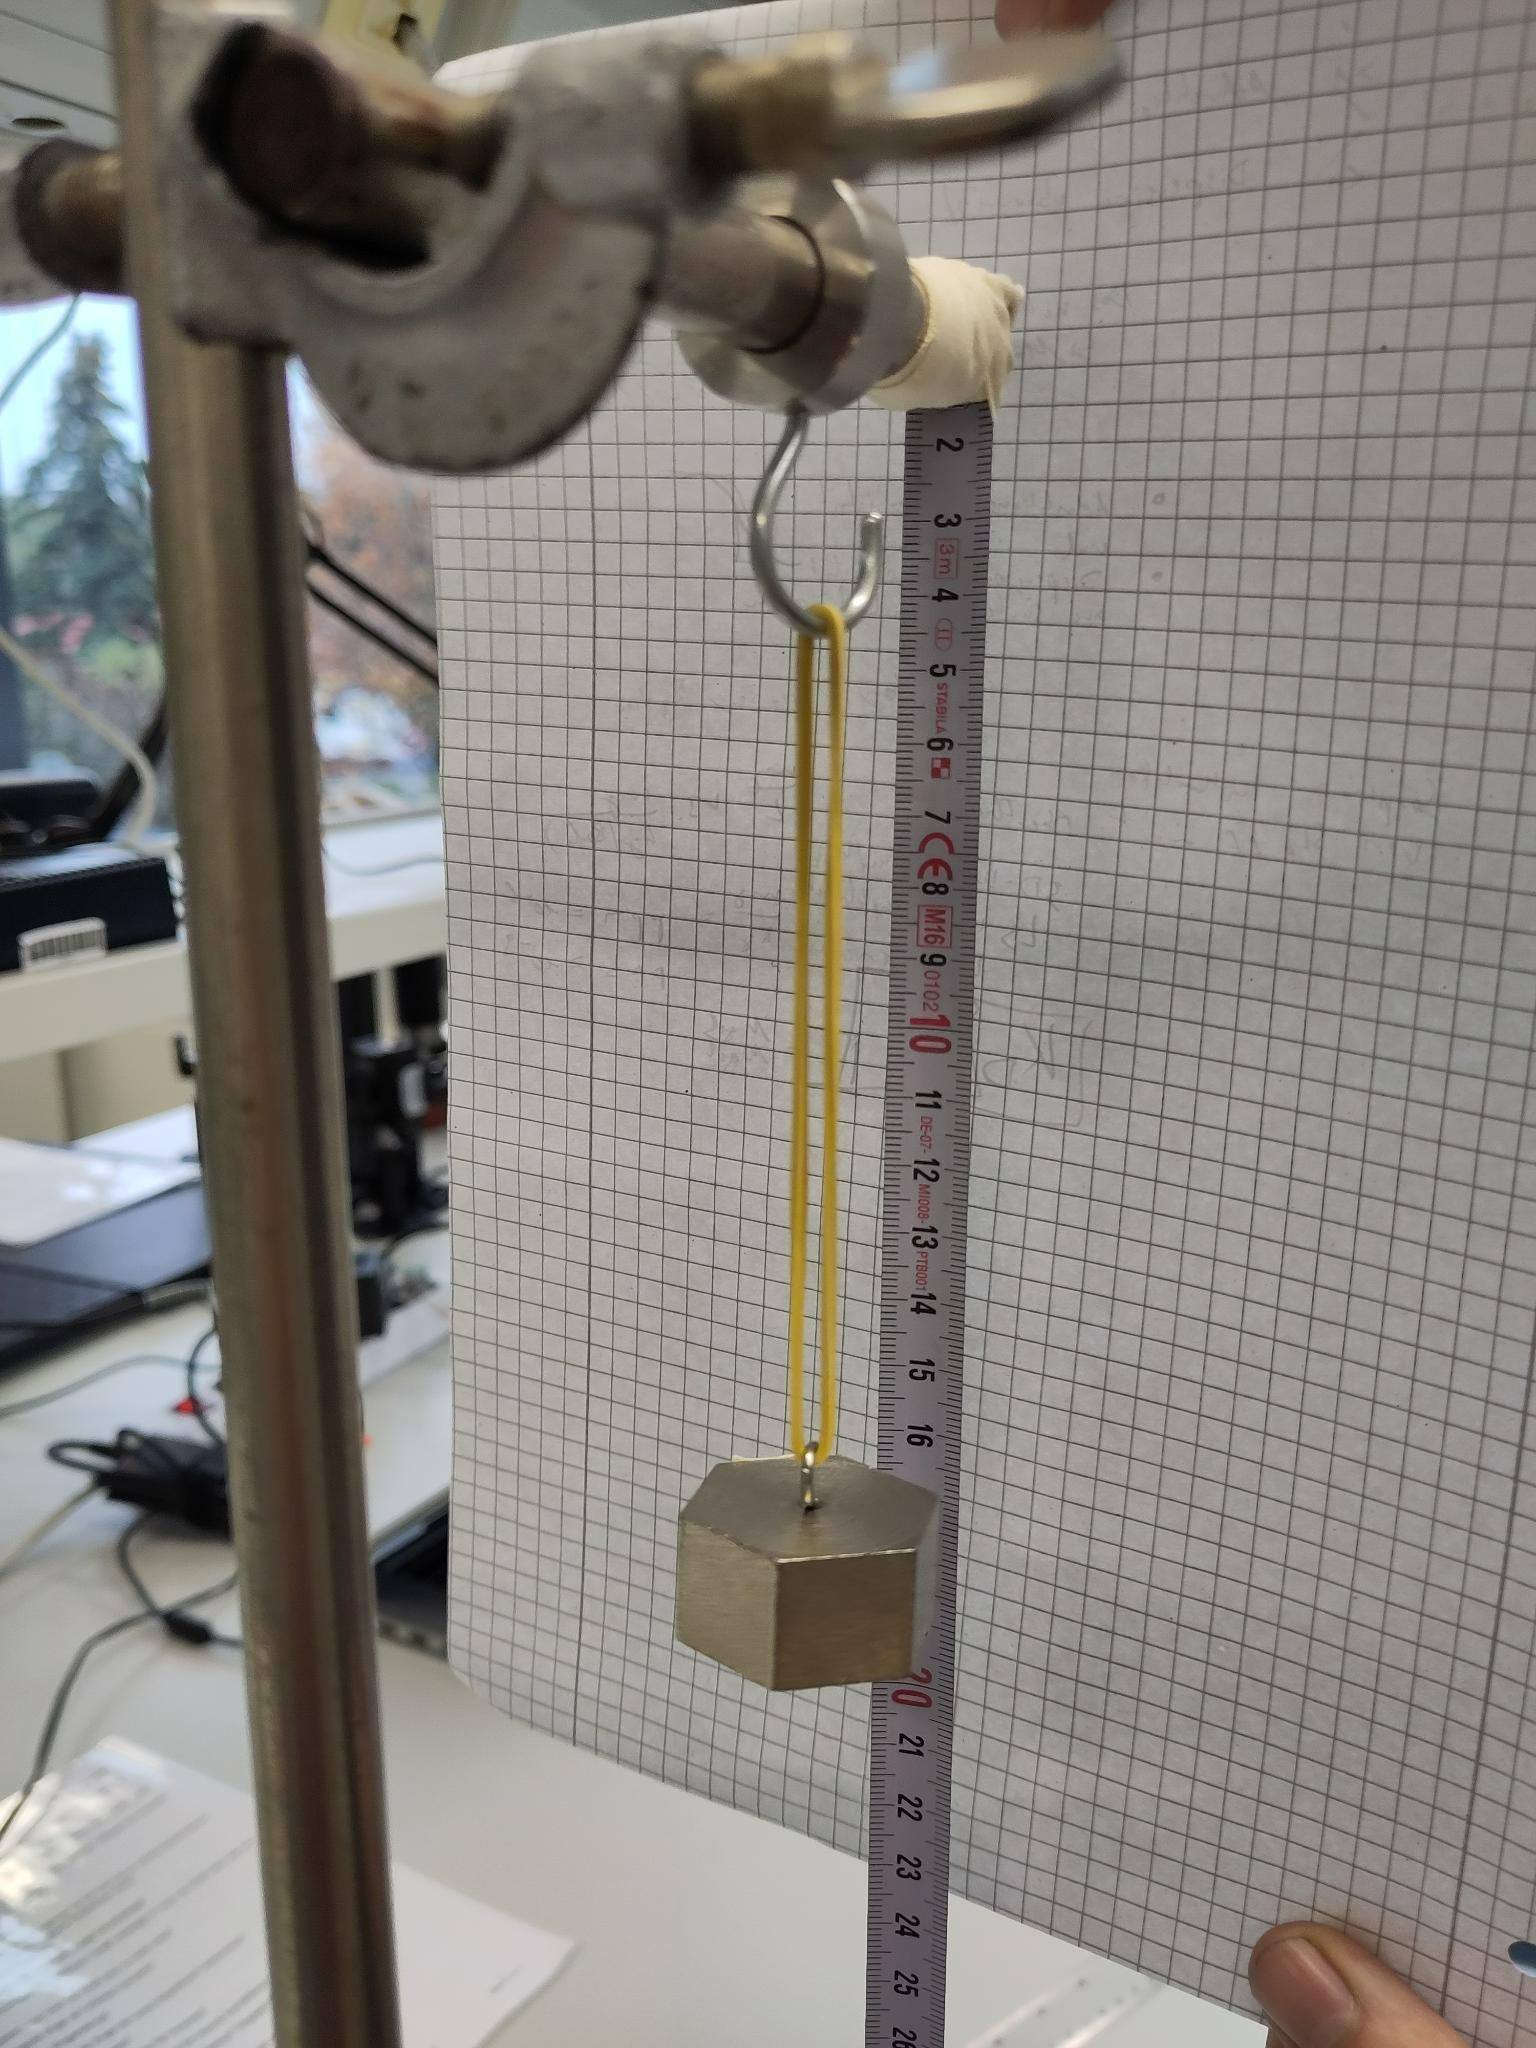
\includegraphics[width=\textwidth,height=0.2\textheight]{Bilder/V1B1.jpeg}
\caption{Versuchsaufbau 1}
\end{figure}

\begin{figure}
\centering
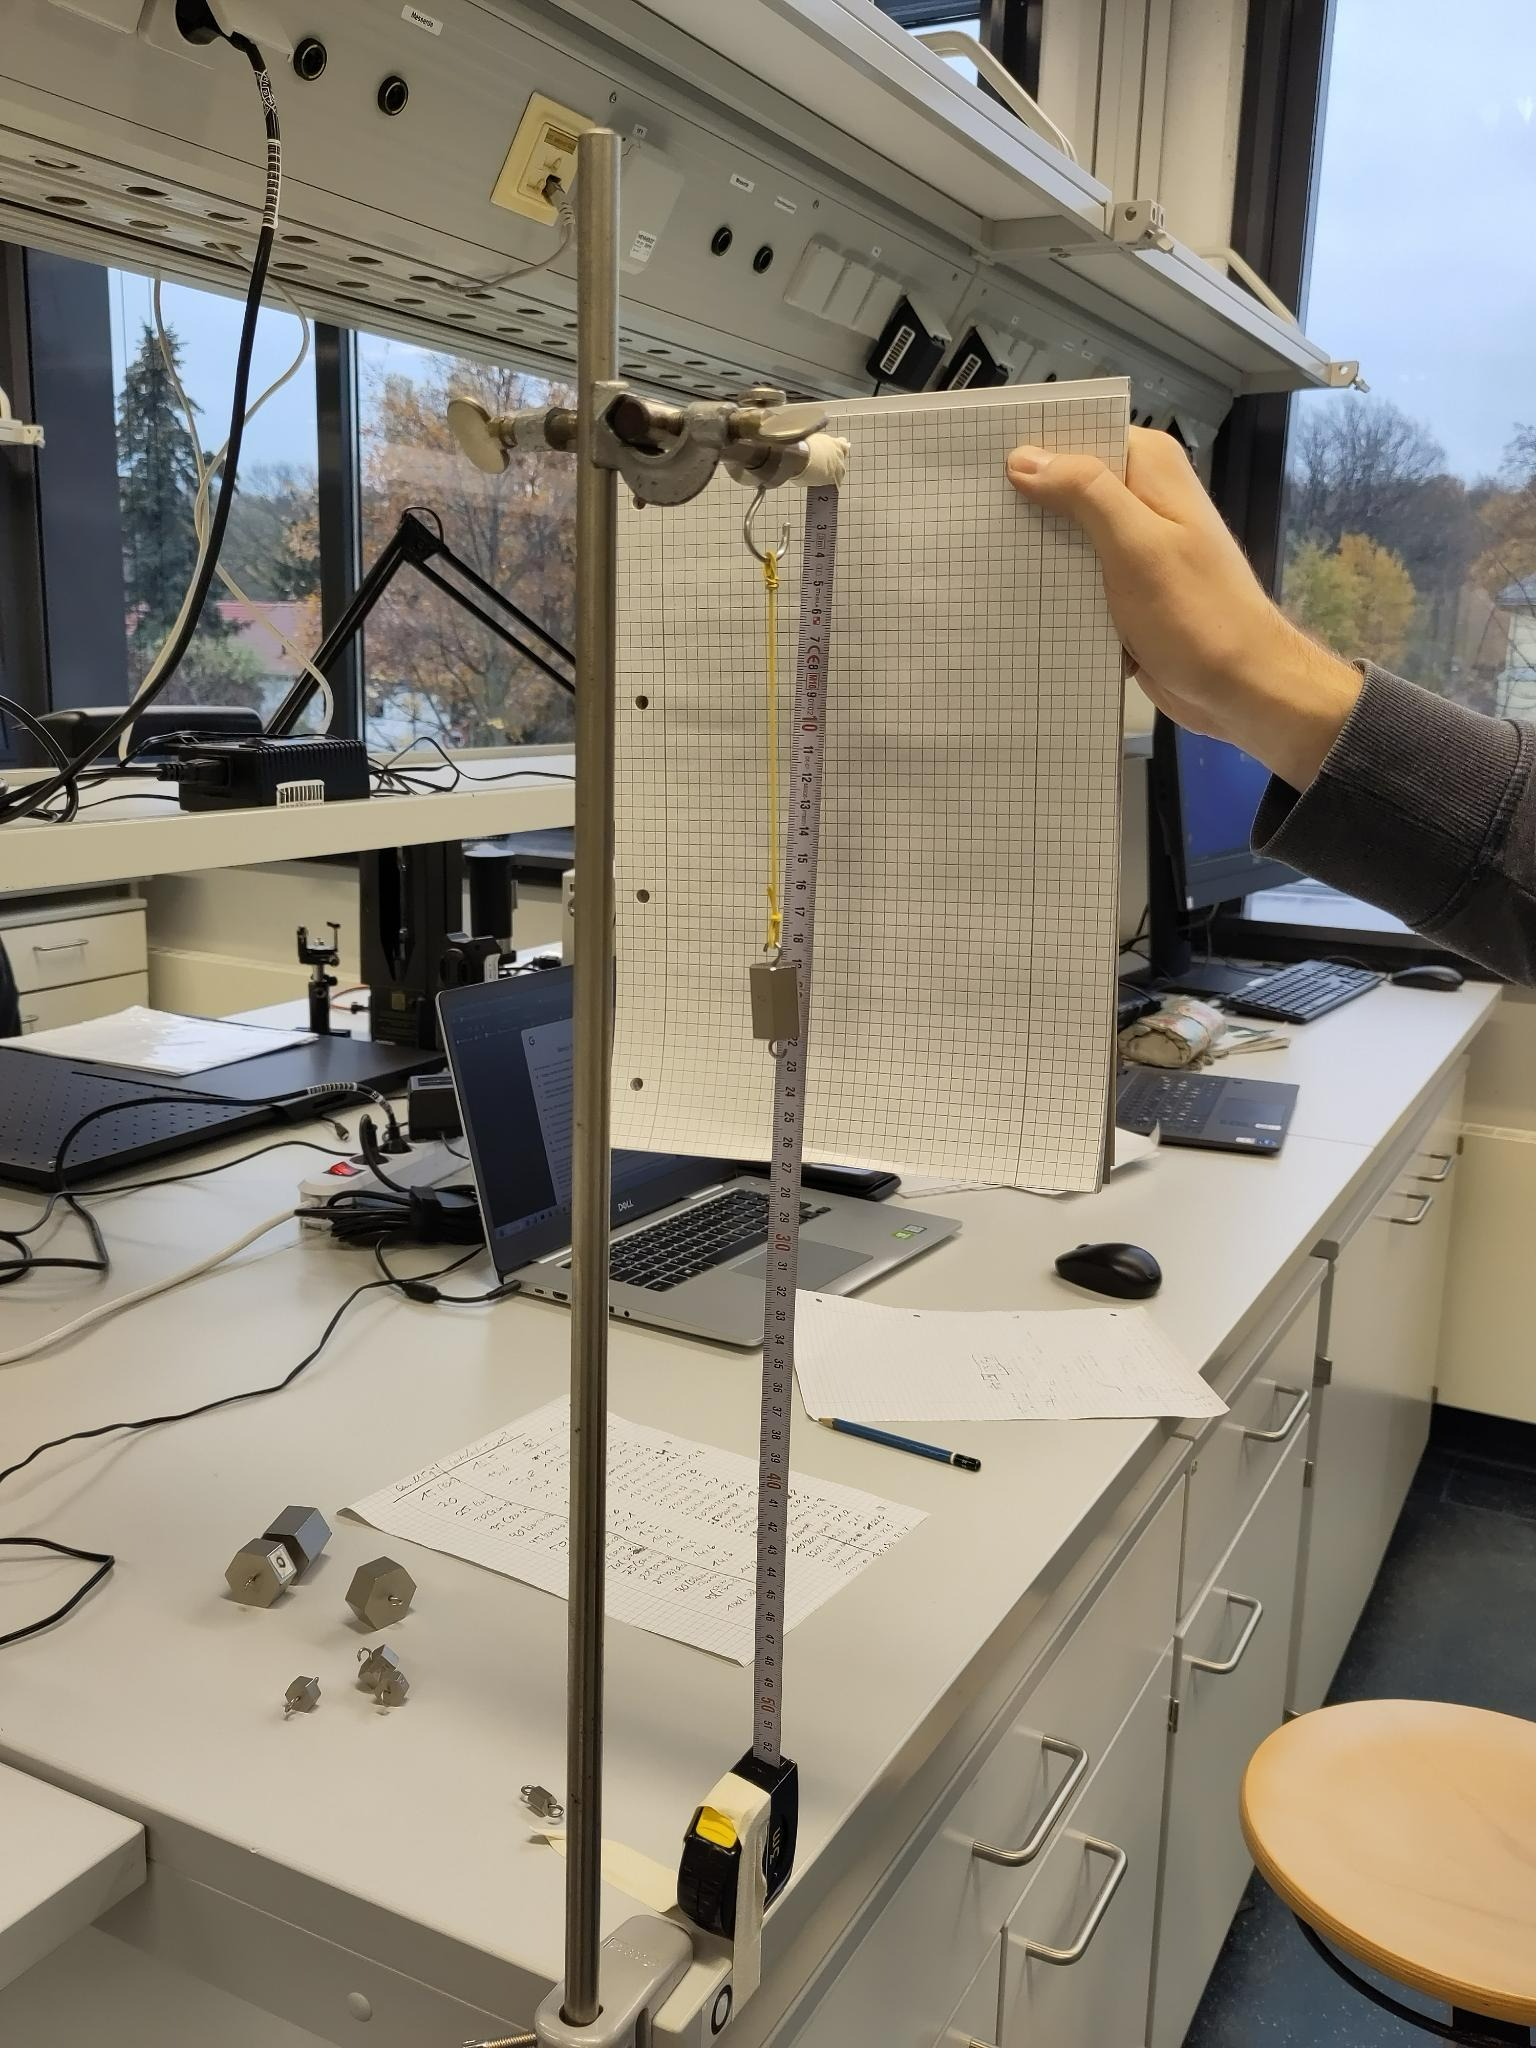
\includegraphics[width=\textwidth,height=0.2\textheight]{Bilder/V2B2.jpeg}
\caption{Versuchsaufbau 1, Nahansicht}
\end{figure}

\hypertarget{durchfuxfchrung}{%
\subsection{Durchführung}\label{durchfuxfchrung}}

Die Gewichte werden gewogen und die Messunsicherheiten berechnet. Die
10g und die 100g Gewichte lagen doppelt vor und waren jeweils gleich
schwer. Die Gewichte stellten sich generell als zu leicht heraus. Nur
die zwei 10g Gewichte wogen nach einer Beschriftung mit Klebeband
\(10,0g\).

\begin{longtable}[]{@{}lr@{}}
\caption{Verwendete Gewichte}\tabularnewline
\toprule()
Nominalgewicht & Einzelmasse\_g \\
\midrule()
\endfirsthead
\toprule()
Nominalgewicht & Einzelmasse\_g \\
\midrule()
\endhead
5g & 4.8 \\
10g (2x) & 10.0 \\
20g & 19.8 \\
50g & 49.9 \\
100g (2x) & 99.5 \\
200g & 198.5 \\
\bottomrule()
\end{longtable}

Die Gesamtmasse \(m_{ges}\) einer Gewichtskombination wird durch
Addition der Teilmassen berechnet.

Die Geräteungenauigkeit berechnet sich zu:
\(u_{Gerät}= \sqrt{u_{Skala}^2+u_{Waage}^2}\). Dabei ist \(u_{Skala}\)
konstant bei \(u_{Skala} = \frac{0,0001kg}{2\sqrt{3}}=2,9*10^{-5}kg\).
Für \(u_{Waage}\) wurde eine Messunsicherheit von \ldots{} am Gerät
abgelesen. Damit errechnet sich eine Geräteungenauigkeit von
\(u_{Gerät}=\) \ldots{} .

Für die Unsicherheit der aus \(n\) Gewichten kombinierten Masse M
\(u_{m}\) gilt, da für alle Messungen die gleiche Waage benutzt wurde,
der Zusammenhang: \[u_m = \sum\limits_{i=1}^{n}u_{m,i} = n*u_{Gerät}\]
Mit \(n\): Anzahl der kombinierten Gewichte

\begin{Shaded}
\begin{Highlighting}[]
\CommentTok{\# Skalenunsicherheit}
\NormalTok{u\_Skala }\OtherTok{=}\NormalTok{ (}\DecValTok{1}\SpecialCharTok{*}\DecValTok{10}\SpecialCharTok{**}\NormalTok{(}\SpecialCharTok{{-}}\DecValTok{4}\NormalTok{))}\SpecialCharTok{/}\NormalTok{(}\DecValTok{2}\SpecialCharTok{*}\FunctionTok{sqrt}\NormalTok{(}\DecValTok{3}\NormalTok{)) }\CommentTok{\#kg}
\CommentTok{\# BAUSTELLE: Hier fehlt noch die Geräteungenauigkeit der Waage (Waagenunsicherheit)}
\NormalTok{u\_Waage }\OtherTok{=} \FloatTok{0.05}\SpecialCharTok{*}\DecValTok{10}\SpecialCharTok{**}\NormalTok{(}\SpecialCharTok{{-}}\DecValTok{3}\NormalTok{) }\CommentTok{\#Geschätzt in kg}
\CommentTok{\# Geräteunsicherheit}
\NormalTok{u\_Gerät }\OtherTok{=} \FunctionTok{sqrt}\NormalTok{((u\_Skala)}\SpecialCharTok{\^{}}\DecValTok{2}\SpecialCharTok{+}\NormalTok{(u\_Waage)}\SpecialCharTok{\^{}}\DecValTok{2}\NormalTok{)}
\CommentTok{\# Massenunsicherheit}
\NormalTok{u\_m }\OtherTok{=}\NormalTok{ Gewichte}\SpecialCharTok{$}\NormalTok{n\_Gewichte}\SpecialCharTok{*}\NormalTok{u\_Gerät }\CommentTok{\#kg}
\end{Highlighting}
\end{Shaded}

Zunächst wird die Länge des Gummibandes ohne zusätzliches Gewicht
gemessen. Die Länge betrug 11,2 cm. Diese Länge muss später von allen
Messwerten abgezogen werden, um nur die Auslenkung aus dem Nullzustand
als Datensatz aufzunehmen.

Danach werden nacheinander verschiedene Gewichte an das Gummiband
gehängt und die entsprechende Elongation gemessen. Diese wird an der
Unterkante des Gummibandes, sobald dieses nach dem Anbringen der
Gewichte nicht mehr schwingt, abgelesen. Unsere Gruppe entschied sich
zunächst dafür, eine Messreihe mit Intervallen von \(5g\) durchzuführen.
Nach den ersten 20 Messungen (\(100g\)) entschieden wir uns dafür, die
Intervalle auf \(10g\) zu erhöhen, da wir zunächst den Aufwand
unterschätzten und Daten mit einem Abstand von 10g immer noch zur
Beurteilung der Federkonstante ausreichen.

Die Auslenkung wird am Maßband abgelesen (Messskala in mm). Dies
bedeutet eine Ungenauigket der Elongation von:
\[u_{x}=\frac{a}{2\sqrt{6}}= \frac{0,001m}{2\sqrt{6}}=2,0*10^{-4}m\]

\begin{Shaded}
\begin{Highlighting}[]
\CommentTok{\# Auslenkungsungenauigkeit }
\NormalTok{u\_x }\OtherTok{=} \FloatTok{2.0}\SpecialCharTok{*}\DecValTok{10}\SpecialCharTok{**}\NormalTok{(}\SpecialCharTok{{-}}\DecValTok{4}\NormalTok{) }\CommentTok{\#m}
\end{Highlighting}
\end{Shaded}

\hypertarget{fehlerquellen}{%
\subsection{Fehlerquellen}\label{fehlerquellen}}

Bei den Fehlerquellen ist zunächst der \textbf{personenbezogene
Ablesefehler} zu erwähnen. Diesen versuchten wir weitestgehend zu
eliminieren, indem nur eine Person eine vollständige Datenreihe aufnahm.

Eine weitere Fehlerquelle kann die \textbf{Zeitabhängigkeit der
Auslenkung} sein. Ein Gummiband kann nach einer gewissen Zeit mehr
nachgeben, als bei der direkten Messung. Wir haben uns bemüht, die
Messungen sehr direkt und ohne Verzug vorzunehmen. Die Zeitanghängigkeit
haben wir jedoch nicht näher untersucht.

Besonders wichtig ist zu erwähnen, dass die Länge \(x_0\) am Anfang und
am Ende nicht übereinstimmten (11,2cm am Anfang zu 11,6cm am Ende). Dies
ist auf die \textbf{konstante Dehnung des Gummibandes} zurückzuführen
und wurde ebenfalls bei der Messung vernachlässigt.

Neben diesen Versuchsbezogenen Fehlerquellen sind Annahmen zu nennen,
die das Hooksche Gesetz trifft. Diese können sich aber in der Realität
anders darstellen. Dabei sind zu nennen:

\begin{itemize}
\tightlist
\item
  Vernachlässigung von Energieumwandlung (z.B.: durch Reibung,
  \(W=F_s*s\))
\item
  Lineare Kraft-Auslenkungs-Beziehung (Speziell im Falle des Gummibandes
  nur eingeschränkt anwendbar)
\item
  Der Stoff soll dehnbar sein, die Elastizitätsgrenze darf jedoch nicht
  überschritten werden.
\item
  Gleiches Verhalten bei und Dehnung und Entspannung der Feder/des
  Gummibandes
\end{itemize}

\hypertarget{messung}{%
\subsection{Messung}\label{messung}}

Mittels Excel werden die Daten aufgenommen und als csv-Datei exportiert.
An dieser Stelle können die erhobenen Messwerte zum Zwecke der
Interpretation aus dieser csv-Datei eingelesen werden. Die Werte sind
auf der letzten Seite aufgeführt, zusammen mit errechneten Größen und
zugehörigen Unsicherheiten.

\begin{Shaded}
\begin{Highlighting}[]
\NormalTok{Messreihe }\OtherTok{\textless{}{-}} \FunctionTok{read.csv}\NormalTok{(}\StringTok{"Daten/Messreihe.csv"}\NormalTok{, }\AttributeTok{sep=}\StringTok{";"}\NormalTok{, }\AttributeTok{dec =} \StringTok{","}\NormalTok{)}

\CommentTok{\# Anbindung der bereits errechneten Unsicherheit der Masse}
\NormalTok{Messreihe }\OtherTok{\textless{}{-}} \FunctionTok{cbind}\NormalTok{(Messreihe, u\_m)}

\FunctionTok{colnames}\NormalTok{(Messreihe) }\OtherTok{\textless{}{-}} \FunctionTok{c}\NormalTok{(}\StringTok{"n\_Gewichte"}\NormalTok{, }\StringTok{"Sollwert\_g"}\NormalTok{, }\StringTok{"Gewicht\_g"}\NormalTok{, }
                         \StringTok{"Auslenkung1\_cm"}\NormalTok{,  }\StringTok{"Auslenkung2"}\NormalTok{, }\StringTok{"x\_Haken"}\NormalTok{, }
                         \StringTok{"x\_0\_Ende"}\NormalTok{, }\StringTok{"u\_m"}\NormalTok{)}
\end{Highlighting}
\end{Shaded}

\hypertarget{auswertung-und-interpretation}{%
\subsection{Auswertung und
Interpretation}\label{auswertung-und-interpretation}}

\hypertarget{berechnung-der-gewichts--und-zugkraft}{%
\subsubsection{Berechnung der Gewichts- und
Zugkraft}\label{berechnung-der-gewichts--und-zugkraft}}

Zur Interpretation der Messergebnisse wird die Elongation \(x_i\)
normiert, indem die Nullauslenkung, diese beträgt \(11,2 cm\) auf dem
Maßband, von den anderen Messwerten subtrahiert wird, siehe
entsprechenden Messwert für ein Gewicht von \(0g\).

Zudem wird, wie bei allen anderen Messgrößen auch, die Einheit in eine
SI-Einheit umgerechnet, um den Einheitenbezug korrekt zu halten. In
diesem Falle also in Meter.

Im Anschluss wird die Kraft \(F_{G,i} = m_i * g\) in Newton berechnet,
die für das Gewicht \(m_i\) auf das Gummiband wirkt. Die
Erdbeschleunigung \(g\) wird auf \(9,81\frac{m}{s^2}\) festgesetzt. Im
Folgenden wird, wenn die Unterscheidung zwischen Gewichts- und Zugkraft
aufgrund der Betragsgleichheit im zu untersuchenden Ruhezustand unsinnig
ist, von einer sematischen Unterscheidung von \(F_G\) und \(F_{Zug}\)
abgesehen und stattdessen verallgemeinernd von der wirkenden Kraft \(F\)
gesprochen. Neben der Kraft \(F\) wird auch die Unsicherheit der Kraft
berechnet. Diese berechnet sich als: \begin{align*}
\begin{split}
u_F &= \frac{\partial F}{\partial {m}}*u_m\\
    &= g*u_m\\
\end{split}
\end{align*}

Nach der Rechnung wird ein Kraft-Auslenkung Schaubild erstellt.

\begin{Shaded}
\begin{Highlighting}[]
\CommentTok{\# Nullwerte(x\_0 = 11,2cm) abziehen}
\NormalTok{Messreihe}\SpecialCharTok{$}\NormalTok{Auslenkung1\_x0 }\OtherTok{\textless{}{-}}\NormalTok{ Messreihe}\SpecialCharTok{$}\NormalTok{Auslenkung1\_cm }\SpecialCharTok{{-}} \FloatTok{11.2}

\CommentTok{\# Einheitenbezug}
\NormalTok{Messreihe}\SpecialCharTok{$}\NormalTok{Gewicht\_kg }\OtherTok{\textless{}{-}}\NormalTok{ Messreihe}\SpecialCharTok{$}\NormalTok{Gewicht\_g}\SpecialCharTok{/}\DecValTok{1000} \CommentTok{\#g {-}\textgreater{} kg}
\NormalTok{Messreihe}\SpecialCharTok{$}\NormalTok{Auslenkung1\_x0\_m }\OtherTok{\textless{}{-}}\NormalTok{  Messreihe}\SpecialCharTok{$}\NormalTok{Auslenkung1\_x0}\SpecialCharTok{/}\DecValTok{100} \CommentTok{\#cm {-}\textgreater{} m}

\CommentTok{\# ERDBESCHLEUNIGUNG}
\NormalTok{g }\OtherTok{=} \FloatTok{9.81} \CommentTok{\#m/s\^{}2}

\CommentTok{\# Berechnung von Kraft und u\_Kraft}
\NormalTok{Messreihe}\SpecialCharTok{$}\NormalTok{Kraft }\OtherTok{\textless{}{-}}\NormalTok{ Messreihe}\SpecialCharTok{$}\NormalTok{Gewicht\_kg }\SpecialCharTok{*}\NormalTok{ g }\CommentTok{\#N}
\NormalTok{Messreihe}\SpecialCharTok{$}\NormalTok{u\_Kraft }\OtherTok{\textless{}{-}}\NormalTok{ g}\SpecialCharTok{*}\NormalTok{u\_m}
\end{Highlighting}
\end{Shaded}

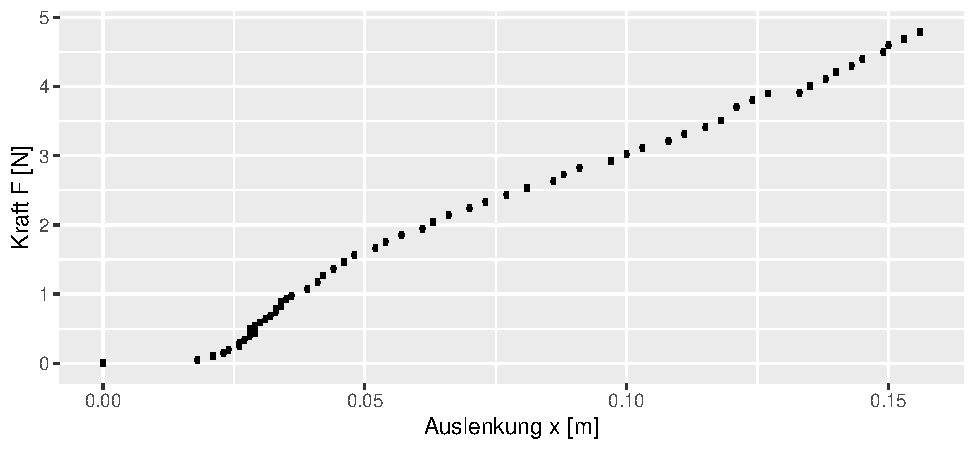
\includegraphics{DehnbareStoffe_files/figure-latex/unnamed-chunk-6-1.pdf}
Wird \(F\) gegen \(x_i\) aufgetragen, ergibt sich optisch ab einer
Auslenkung von \(5cm\) ein etwa linearer Zusammenhang. Im Bereich
zwischen einer Elongation von \(0cm\) und \(5cm\) kann das
Ausdehnungsverhalten des Gummibandes unter einer Gewichtsbelastung nicht
als linear betrachtet und nicht durch eine Federkonstante beschrieben
werden. Für die Berechnung der Federkonstanten haben wir uns daher
entschieden, die Werte für \(x_i<0,05m\) auszuschließen. Zugleich müssen
wir dann allerdings feststellen, dass die errechnete Federkonstante nur
im Intervall \(x \in (0,05m,\ x_{max}]\) gilt.

\hypertarget{berechnung-der-federkonstanten}{%
\subsubsection{Berechnung der
Federkonstanten}\label{berechnung-der-federkonstanten}}

Da die Gewichtskraft \(F_G=m*g\) und die Zugkraft des Gummibandes
\(F_{Zug} = x * D\) im Ruhezustand im Gleichgewicht zueinander stehen,
gilt folgende Formel:

\[F_G = m * g = D*x = F_{Zug}\]

Mit:

\begin{itemize}
\tightlist
\item
  \(D\): Federkonstante
\item
  \(m\): Masse des Gewichtes,
\item
  \(x\): Auslenkung,
\item
  \(g\): Erdbeschleunigung (\(9,81\frac{m}{s^2}\)).
\end{itemize}

Daraus ergibt sich für die Federkonstante D:
\begin{equation}\label{hook:eq:Federkonstante}
  D =\frac{m*g}{x}
\end{equation}

Diese wird für jede Auslenkung \(x_i\) berechnet.

\begin{Shaded}
\begin{Highlighting}[]
\NormalTok{Messreihe}\SpecialCharTok{$}\NormalTok{Federkonstante }\OtherTok{\textless{}{-}}\NormalTok{ Messreihe}\SpecialCharTok{$}\NormalTok{Gewicht\_kg}\SpecialCharTok{*}\NormalTok{g}\SpecialCharTok{/}\NormalTok{Messreihe}\SpecialCharTok{$}\NormalTok{Auslenkung1\_x0\_m}
\end{Highlighting}
\end{Shaded}

Die Unsicherheit der einzelnen Werte der Federkonstanten \(u_D\) ergibt
sich gemäß der Gaussschen-Fehlerfortpflanzung aus folgender Formel:

\begin{equation}\label{hook:eq:u_Federkonstante}
\begin{split}
u_D &= \sqrt{(\frac{\partial{D}}{\partial{m}}*u_m)^2+(\frac{\partial{D}}{\partial{x}}*u_x)^2}\\
u_D &=\sqrt{(\frac{g}{x}*u_m)^2+(-\frac{m*g}{x^2}*u_x)^2}\\
\end{split}
\end{equation}

Berechnung in R:

\begin{Shaded}
\begin{Highlighting}[]
\CommentTok{\# Funktion zur Berechnung der Messunsicherheit der Federkonstanten}
\CommentTok{\# INPUT: x, m, u\_m, u\_x (glob)}
\CommentTok{\# OUTPUT: u\_D}
\NormalTok{u\_D\_funktion }\OtherTok{\textless{}{-}} \ControlFlowTok{function}\NormalTok{(x,m, UM)\{}
  \FunctionTok{sqrt}\NormalTok{(((g}\SpecialCharTok{/}\NormalTok{x)}\SpecialCharTok{*}\NormalTok{UM)}\SpecialCharTok{**}\DecValTok{2}\SpecialCharTok{+}\NormalTok{((}\SpecialCharTok{{-}}\NormalTok{m}\SpecialCharTok{*}\NormalTok{g}\SpecialCharTok{/}\NormalTok{x}\SpecialCharTok{**}\DecValTok{2}\NormalTok{)}\SpecialCharTok{*}\NormalTok{u\_x)}\SpecialCharTok{**}\DecValTok{2}\NormalTok{)}
\NormalTok{\}}

\CommentTok{\# Berechnung der Unsicherheit der Federkonstanten}
\NormalTok{Messreihe}\SpecialCharTok{$}\NormalTok{u\_Federkonstante }\OtherTok{\textless{}{-}} \FunctionTok{u\_D\_funktion}\NormalTok{(}\AttributeTok{x=}\NormalTok{Messreihe}\SpecialCharTok{$}\NormalTok{Auslenkung1\_x0\_m, }
                                           \AttributeTok{m=}\NormalTok{Messreihe}\SpecialCharTok{$}\NormalTok{Gewicht\_kg,}
                                           \AttributeTok{UM=}\NormalTok{Messreihe}\SpecialCharTok{$}\NormalTok{u\_m)}
\end{Highlighting}
\end{Shaded}

Wird die Federkonstante über die Elongation geplottet, zeigt sich
wieder, dass diese erst ab einer Auslenkung von etwa 5 cm einen
vergleichsweise Stabilen Wert annimmt.

\begin{center}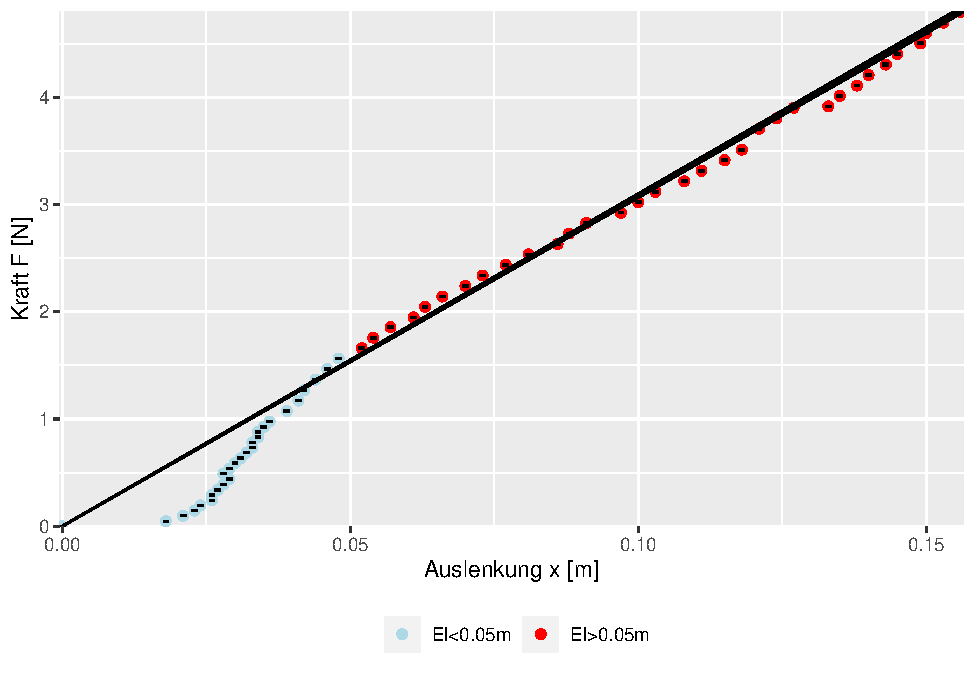
\includegraphics{DehnbareStoffe_files/figure-latex/unnamed-chunk-9-1} \end{center}

Daher haben wir uns entschiden, nur in dem beschriebenen Intervall
\(x \in (0,05m,\ x_{max}]\) zu mitteln. Dort wird nach GUM der
Mittelwert und die Standardabweichung des Mittelwertes berechnet, um ein
Messergebnis und dessen Unsicherheit zu erhalten.

Mittelwert: \begin{equation}\label{Mittelwert}
\overline{D} = \frac{1}{n}\sum \limits_{i=1}^nD_i
\end{equation}

Standardabweichung: \begin{equation}\label{Standardabweichung}
\sigma_D = \sqrt{\frac{1}{n-1} \sum_{i=1}^n (D_i - \overline{D})^2}
\end{equation}

Standardabweichung des Mittelwertes:
\begin{equation}\label{StandardabweichungDesMittelwertes}
\sigma_{\overline{D}}=\frac{\sigma_D}{\sqrt{n}}
\end{equation}

\begin{longtable}[]{@{}lr@{}}
\caption{Statistische Größen zur bestimmten
Federkonstante}\tabularnewline
\toprule()
& Werte \\
\midrule()
\endfirsthead
\toprule()
& Werte \\
\midrule()
\endhead
Mittelwert\_MW & 30.8162757 \\
Standardabweichung\_SD & 0.9579652 \\
SD\_von\_MW & 0.1667603 \\
\bottomrule()
\end{longtable}

Die bestimmte Federkonstante, für eine Auslenkung des Gummibandes im
Bereich von \(5,0\) bis \(26.8cm\), beträgt also
\(D_1=(30,82\pm 0,17)\frac{N}{m}\)

\newpage

Hier wird die Federkonstante als Gerade nocheinmal im
Kraft-Auslenkungsschaubild dargestellt. Die blau eingefärbten Punkte
sind diejenigen Punkte, die nicht in die Berechnung mit eingingen.

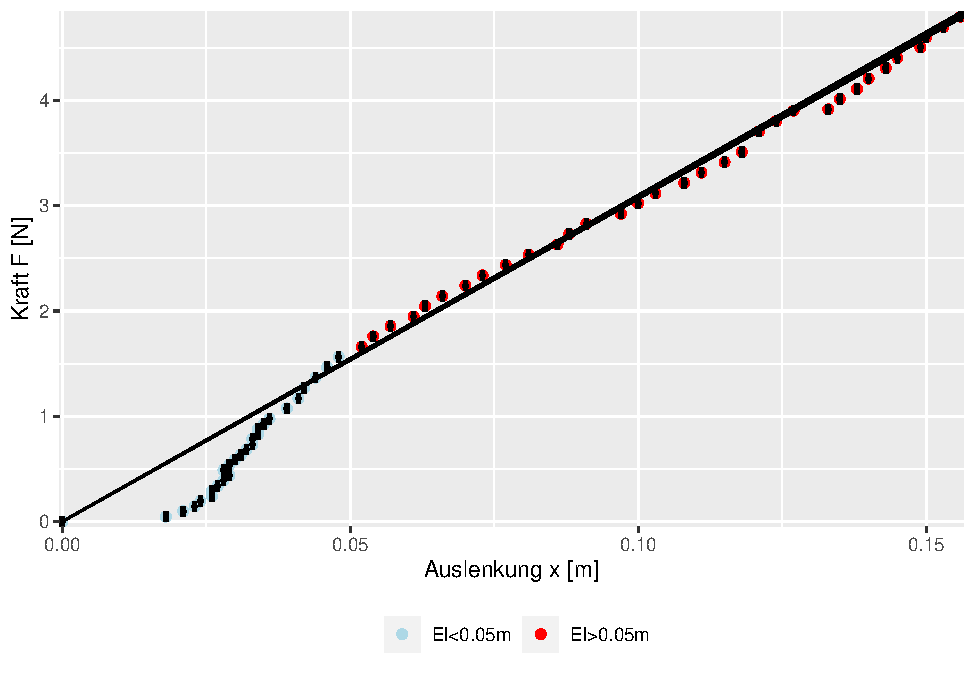
\includegraphics{DehnbareStoffe_files/figure-latex/unnamed-chunk-11-1.pdf}
Angemerkt sei, dass für die Steigung der Federkonstanten der Mittelwert
und die Mittelwerte ab- bzw. zuzüglich der Standardabweichung des
Mittelwertes angenommen wurden. Die Drei Geraden überlagern sich sehr
stark. Ebenso wurde ein Nulldurchgang festgelegt, da bei keiner
Krafteinwirkung keine Elongation stattfindet. Ebenso sei angemerkt, dass
die Fehlerbalken vorhanden sind, wie auch in den Diagrammen zuvor, nur
dass diese eher klein ausfallen, vergleiche entsprechend errechnete
Werte im Abschnitt \textit{Messwerte und errechnete Größen}.

\hypertarget{messwerte-und-errechnete-gruxf6uxdfen}{%
\subsubsection{Messwerte und errechnete
Größen}\label{messwerte-und-errechnete-gruxf6uxdfen}}

Im Folgenden eine Auflistung der in diesem Versuch erhobenen Messwerte
und der daraus errechneten Größen:

Mit:

\begin{itemize}
\tightlist
\item
  n\_m{[}-{]}: Anzahl kombinierter Gewichte
\item
  m{[}kg{]}: Masse der kombinierten Gewichte in Kilogramm
\item
  u\_m{[}kg{]}: Unsicherheit der Masse in Kilogramm
\item
  L{[}cm{]}: Abgelesener Wert an Maßband in Zentimeter
\item
  El{[}m{]}: Elongation des Gummibandes in Meter
\item
  F{[}N{]}: Kraft F in Newton
\item
  u\_F{[}N{]}: Unsicherheit der Kraft in Newton
\item
  D{[}N/m{]}: Federkonstante D in Newton pro Meter
\item
  u\_D{[}N/m{]}: Unsicherheit der Federkonstante in Newton pro Meter
\end{itemize}

\begin{longtable}[]{@{}
  >{\raggedleft\arraybackslash}p{(\columnwidth - 16\tabcolsep) * \real{0.1029}}
  >{\raggedleft\arraybackslash}p{(\columnwidth - 16\tabcolsep) * \real{0.1029}}
  >{\raggedleft\arraybackslash}p{(\columnwidth - 16\tabcolsep) * \real{0.1471}}
  >{\raggedleft\arraybackslash}p{(\columnwidth - 16\tabcolsep) * \real{0.0882}}
  >{\raggedleft\arraybackslash}p{(\columnwidth - 16\tabcolsep) * \real{0.0882}}
  >{\raggedleft\arraybackslash}p{(\columnwidth - 16\tabcolsep) * \real{0.1029}}
  >{\raggedleft\arraybackslash}p{(\columnwidth - 16\tabcolsep) * \real{0.1176}}
  >{\raggedleft\arraybackslash}p{(\columnwidth - 16\tabcolsep) * \real{0.1176}}
  >{\raggedleft\arraybackslash}p{(\columnwidth - 16\tabcolsep) * \real{0.1324}}@{}}
\caption{Messwerte}\tabularnewline
\toprule()
\begin{minipage}[b]{\linewidth}\raggedleft
n\_m{[}-{]}
\end{minipage} & \begin{minipage}[b]{\linewidth}\raggedleft
m{[}kg{]}
\end{minipage} & \begin{minipage}[b]{\linewidth}\raggedleft
u\_m{[}kg{]}
\end{minipage} & \begin{minipage}[b]{\linewidth}\raggedleft
L{[}cm{]}
\end{minipage} & \begin{minipage}[b]{\linewidth}\raggedleft
El{[}m{]}
\end{minipage} & \begin{minipage}[b]{\linewidth}\raggedleft
F{[}N{]}
\end{minipage} & \begin{minipage}[b]{\linewidth}\raggedleft
u\_F{[}N{]}
\end{minipage} & \begin{minipage}[b]{\linewidth}\raggedleft
D{[}N/m{]}
\end{minipage} & \begin{minipage}[b]{\linewidth}\raggedleft
u\_D{[}N/m{]}
\end{minipage} \\
\midrule()
\endfirsthead
\toprule()
\begin{minipage}[b]{\linewidth}\raggedleft
n\_m{[}-{]}
\end{minipage} & \begin{minipage}[b]{\linewidth}\raggedleft
m{[}kg{]}
\end{minipage} & \begin{minipage}[b]{\linewidth}\raggedleft
u\_m{[}kg{]}
\end{minipage} & \begin{minipage}[b]{\linewidth}\raggedleft
L{[}cm{]}
\end{minipage} & \begin{minipage}[b]{\linewidth}\raggedleft
El{[}m{]}
\end{minipage} & \begin{minipage}[b]{\linewidth}\raggedleft
F{[}N{]}
\end{minipage} & \begin{minipage}[b]{\linewidth}\raggedleft
u\_F{[}N{]}
\end{minipage} & \begin{minipage}[b]{\linewidth}\raggedleft
D{[}N/m{]}
\end{minipage} & \begin{minipage}[b]{\linewidth}\raggedleft
u\_D{[}N/m{]}
\end{minipage} \\
\midrule()
\endhead
0 & 0.0000 & 0.0000000 & 11.2 & 0.000 & 0.0000 & 0.00000 & NaN & NaN \\
1 & 0.0048 & 0.0000577 & 13.0 & 0.018 & 0.0471 & 0.00057 & 2.6160 &
0.0428 \\
1 & 0.0100 & 0.0000577 & 13.3 & 0.021 & 0.0981 & 0.00057 & 4.6714 &
0.0520 \\
2 & 0.0148 & 0.0001155 & 13.5 & 0.023 & 0.1452 & 0.00113 & 6.3125 &
0.0737 \\
1 & 0.0198 & 0.0000577 & 13.6 & 0.024 & 0.1942 & 0.00057 & 8.0932 &
0.0715 \\
2 & 0.0246 & 0.0001155 & 13.8 & 0.026 & 0.2413 & 0.00113 & 9.2818 &
0.0836 \\
2 & 0.0298 & 0.0001155 & 13.8 & 0.026 & 0.2923 & 0.00113 & 11.2438 &
0.0968 \\
3 & 0.0346 & 0.0001732 & 13.9 & 0.027 & 0.3394 & 0.00170 & 12.5713 &
0.1124 \\
3 & 0.0398 & 0.0001732 & 14.0 & 0.028 & 0.3904 & 0.00170 & 13.9442 &
0.1166 \\
4 & 0.0446 & 0.0002309 & 14.1 & 0.029 & 0.4375 & 0.00227 & 15.0871 &
0.1301 \\
1 & 0.0499 & 0.0000577 & 14.0 & 0.028 & 0.4895 & 0.00057 & 17.4828 &
0.1265 \\
2 & 0.0547 & 0.0001155 & 14.1 & 0.029 & 0.5366 & 0.00113 & 18.5037 &
0.1335 \\
2 & 0.0599 & 0.0001155 & 14.2 & 0.030 & 0.5876 & 0.00113 & 19.5873 &
0.1359 \\
3 & 0.0647 & 0.0001732 & 14.3 & 0.031 & 0.6347 & 0.00170 & 20.4744 &
0.1430 \\
2 & 0.0699 & 0.0001155 & 14.4 & 0.032 & 0.6857 & 0.00113 & 21.4287 &
0.1385 \\
3 & 0.0747 & 0.0001732 & 14.5 & 0.033 & 0.7328 & 0.00170 & 22.2063 &
0.1441 \\
3 & 0.0797 & 0.0001732 & 14.5 & 0.033 & 0.7819 & 0.00170 & 23.6926 &
0.1525 \\
4 & 0.0845 & 0.0002309 & 14.6 & 0.034 & 0.8289 & 0.00227 & 24.3807 &
0.1581 \\
4 & 0.0897 & 0.0002309 & 14.6 & 0.034 & 0.8800 & 0.00227 & 25.8811 &
0.1662 \\
5 & 0.0945 & 0.0002887 & 14.7 & 0.035 & 0.9270 & 0.00283 & 26.4870 &
0.1716 \\
1 & 0.0995 & 0.0000577 & 14.8 & 0.036 & 0.9761 & 0.00057 & 27.1137 &
0.1515 \\
2 & 0.1095 & 0.0001155 & 15.1 & 0.039 & 1.0742 & 0.00113 & 27.5435 &
0.1442 \\
2 & 0.1193 & 0.0001155 & 15.3 & 0.041 & 1.1703 & 0.00113 & 28.5447 &
0.1420 \\
3 & 0.1293 & 0.0001732 & 15.4 & 0.042 & 1.2684 & 0.00170 & 30.2008 &
0.1494 \\
4 & 0.1393 & 0.0002309 & 15.6 & 0.044 & 1.3665 & 0.00227 & 31.0576 &
0.1503 \\
2 & 0.1494 & 0.0001155 & 15.8 & 0.046 & 1.4656 & 0.00113 & 31.8612 &
0.1407 \\
3 & 0.1594 & 0.0001732 & 16.0 & 0.048 & 1.5637 & 0.00170 & 32.5774 &
0.1403 \\
3 & 0.1692 & 0.0001732 & 16.4 & 0.052 & 1.6599 & 0.00170 & 31.9202 &
0.1270 \\
4 & 0.1792 & 0.0002309 & 16.6 & 0.054 & 1.7580 & 0.00227 & 32.5547 &
0.1277 \\
5 & 0.1892 & 0.0002887 & 16.9 & 0.057 & 1.8561 & 0.00283 & 32.5623 &
0.1246 \\
1 & 0.1985 & 0.0000577 & 17.3 & 0.061 & 1.9473 & 0.00057 & 31.9227 &
0.1051 \\
2 & 0.2085 & 0.0001155 & 17.5 & 0.063 & 2.0454 & 0.00113 & 32.4664 &
0.1046 \\
2 & 0.2183 & 0.0001155 & 17.8 & 0.066 & 2.1415 & 0.00113 & 32.4473 &
0.0998 \\
3 & 0.2283 & 0.0001732 & 18.2 & 0.070 & 2.2396 & 0.00170 & 31.9946 &
0.0946 \\
4 & 0.2383 & 0.0002309 & 18.5 & 0.073 & 2.3377 & 0.00227 & 32.0236 &
0.0931 \\
2 & 0.2484 & 0.0001155 & 18.9 & 0.077 & 2.4368 & 0.00113 & 31.6468 &
0.0835 \\
3 & 0.2584 & 0.0001732 & 19.3 & 0.081 & 2.5349 & 0.00170 & 31.2951 &
0.0801 \\
3 & 0.2682 & 0.0001732 & 19.8 & 0.086 & 2.6310 & 0.00170 & 30.5935 &
0.0738 \\
4 & 0.2782 & 0.0002309 & 20.0 & 0.088 & 2.7291 & 0.00227 & 31.0130 &
0.0750 \\
5 & 0.2882 & 0.0002887 & 20.3 & 0.091 & 2.8272 & 0.00283 & 31.0686 &
0.0750 \\
2 & 0.2980 & 0.0001155 & 20.9 & 0.097 & 2.9234 & 0.00113 & 30.1379 &
0.0632 \\
3 & 0.3080 & 0.0001732 & 21.2 & 0.100 & 3.0215 & 0.00170 & 30.2148 &
0.0628 \\
3 & 0.3178 & 0.0001732 & 21.5 & 0.103 & 3.1176 & 0.00170 & 30.2681 &
0.0610 \\
4 & 0.3278 & 0.0002309 & 22.0 & 0.108 & 3.2157 & 0.00227 & 29.7752 &
0.0590 \\
5 & 0.3378 & 0.0002887 & 22.3 & 0.111 & 3.3138 & 0.00283 & 29.8542 &
0.0595 \\
3 & 0.3479 & 0.0001732 & 22.7 & 0.115 & 3.4129 & 0.00170 & 29.6774 &
0.0537 \\
4 & 0.3579 & 0.0002309 & 23.0 & 0.118 & 3.5110 & 0.00227 & 29.7542 &
0.0540 \\
4 & 0.3777 & 0.0002309 & 23.3 & 0.121 & 3.7052 & 0.00227 & 30.6218 &
0.0540 \\
5 & 0.3877 & 0.0002887 & 23.6 & 0.124 & 3.8033 & 0.00283 & 30.6721 &
0.0545 \\
6 & 0.3977 & 0.0003464 & 23.9 & 0.127 & 3.9014 & 0.00340 & 30.7200 &
0.0553 \\
4 & 0.3990 & 0.0002309 & 24.5 & 0.133 & 3.9142 & 0.00227 & 29.4300 &
0.0474 \\
5 & 0.4090 & 0.0002887 & 24.7 & 0.135 & 4.0123 & 0.00283 & 29.7207 &
0.0488 \\
5 & 0.4188 & 0.0002887 & 25.0 & 0.138 & 4.1084 & 0.00283 & 29.7712 &
0.0478 \\
6 & 0.4288 & 0.0003464 & 25.2 & 0.140 & 4.2065 & 0.00340 & 30.0466 &
0.0493 \\
7 & 0.4388 & 0.0004041 & 25.5 & 0.143 & 4.3046 & 0.00396 & 30.1023 &
0.0504 \\
5 & 0.4489 & 0.0002887 & 25.7 & 0.145 & 4.4037 & 0.00283 & 30.3704 &
0.0462 \\
6 & 0.4589 & 0.0003464 & 26.1 & 0.149 & 4.5018 & 0.00340 & 30.2135 &
0.0465 \\
6 & 0.4687 & 0.0003464 & 26.2 & 0.150 & 4.5979 & 0.00340 & 30.6530 &
0.0467 \\
7 & 0.4787 & 0.0004041 & 26.5 & 0.153 & 4.6960 & 0.00396 & 30.6931 &
0.0478 \\
8 & 0.4887 & 0.0004619 & 26.8 & 0.156 & 4.7941 & 0.00453 & 30.7317 &
0.0489 \\
\bottomrule()
\end{longtable}

\hypertarget{versuch-2}{%
\section{Versuch 2}\label{versuch-2}}

\hypertarget{ziel-1}{%
\subsection{Ziel}\label{ziel-1}}

Untersuchung der Fragestellung, ob sich der Zusammenhang zwischen Kraft
und Elongation verändert, wenn man die Angrifffskraft auf einen Strang
des Gummibandes anstatt auf zwei verteilt.

Eine Hypothese ist, dass die Auslenkung bei gleicher Gewichtskraft
doppelt so hoch ist, weil die Kraft auf nur einen Strang wirkt.

\hypertarget{materialien-1}{%
\subsection{Materialien}\label{materialien-1}}

\begin{itemize}
\tightlist
\item
  Stativ
\item
  Gummiband
\item
  Gewichte
\item
  Maßband
\item
  Haken
\item
  Klebeband
\item
  Schere
\end{itemize}

\hypertarget{versuchsaufbau-1}{%
\subsection{Versuchsaufbau}\label{versuchsaufbau-1}}

\begin{itemize}
\tightlist
\item
  Analog zu Versuch 1, aber das Gummiband wurde vorher mit einer Schere
  zerschnitten und durch geknotete Schlaufen an Haken und Gewicht
  befestigt.
\end{itemize}

\begin{figure}
\centering
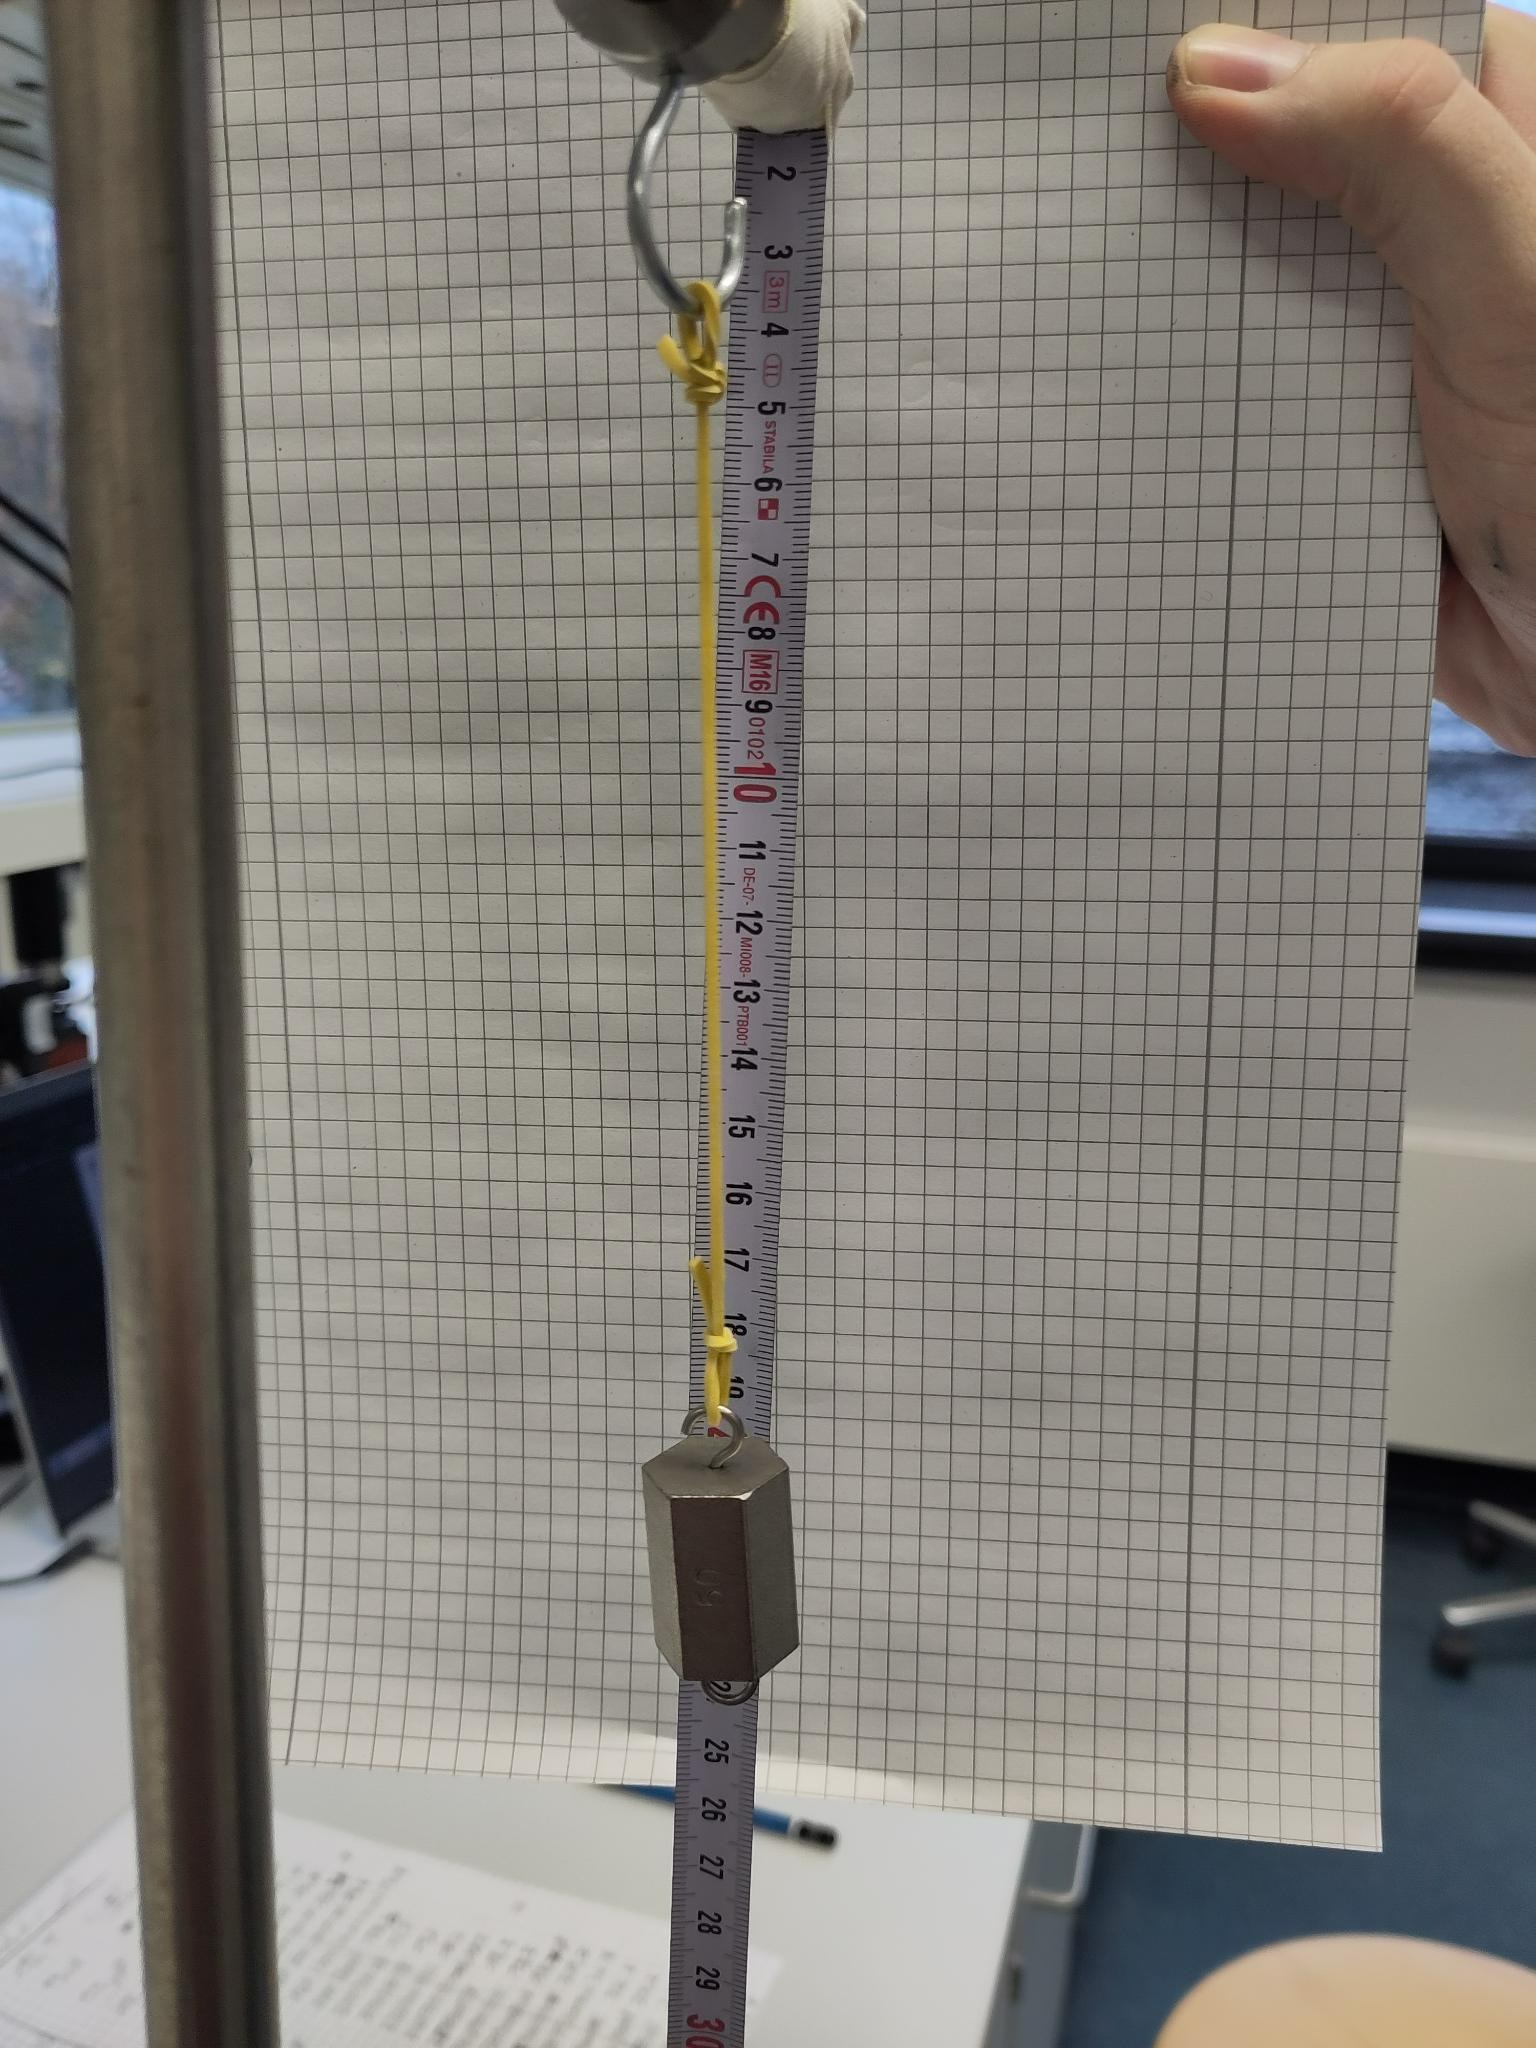
\includegraphics[width=\textwidth,height=0.2\textheight]{Bilder/V2B1.jpeg}
\caption{Versuchsaufbau 2}
\end{figure}

\begin{figure}
\centering
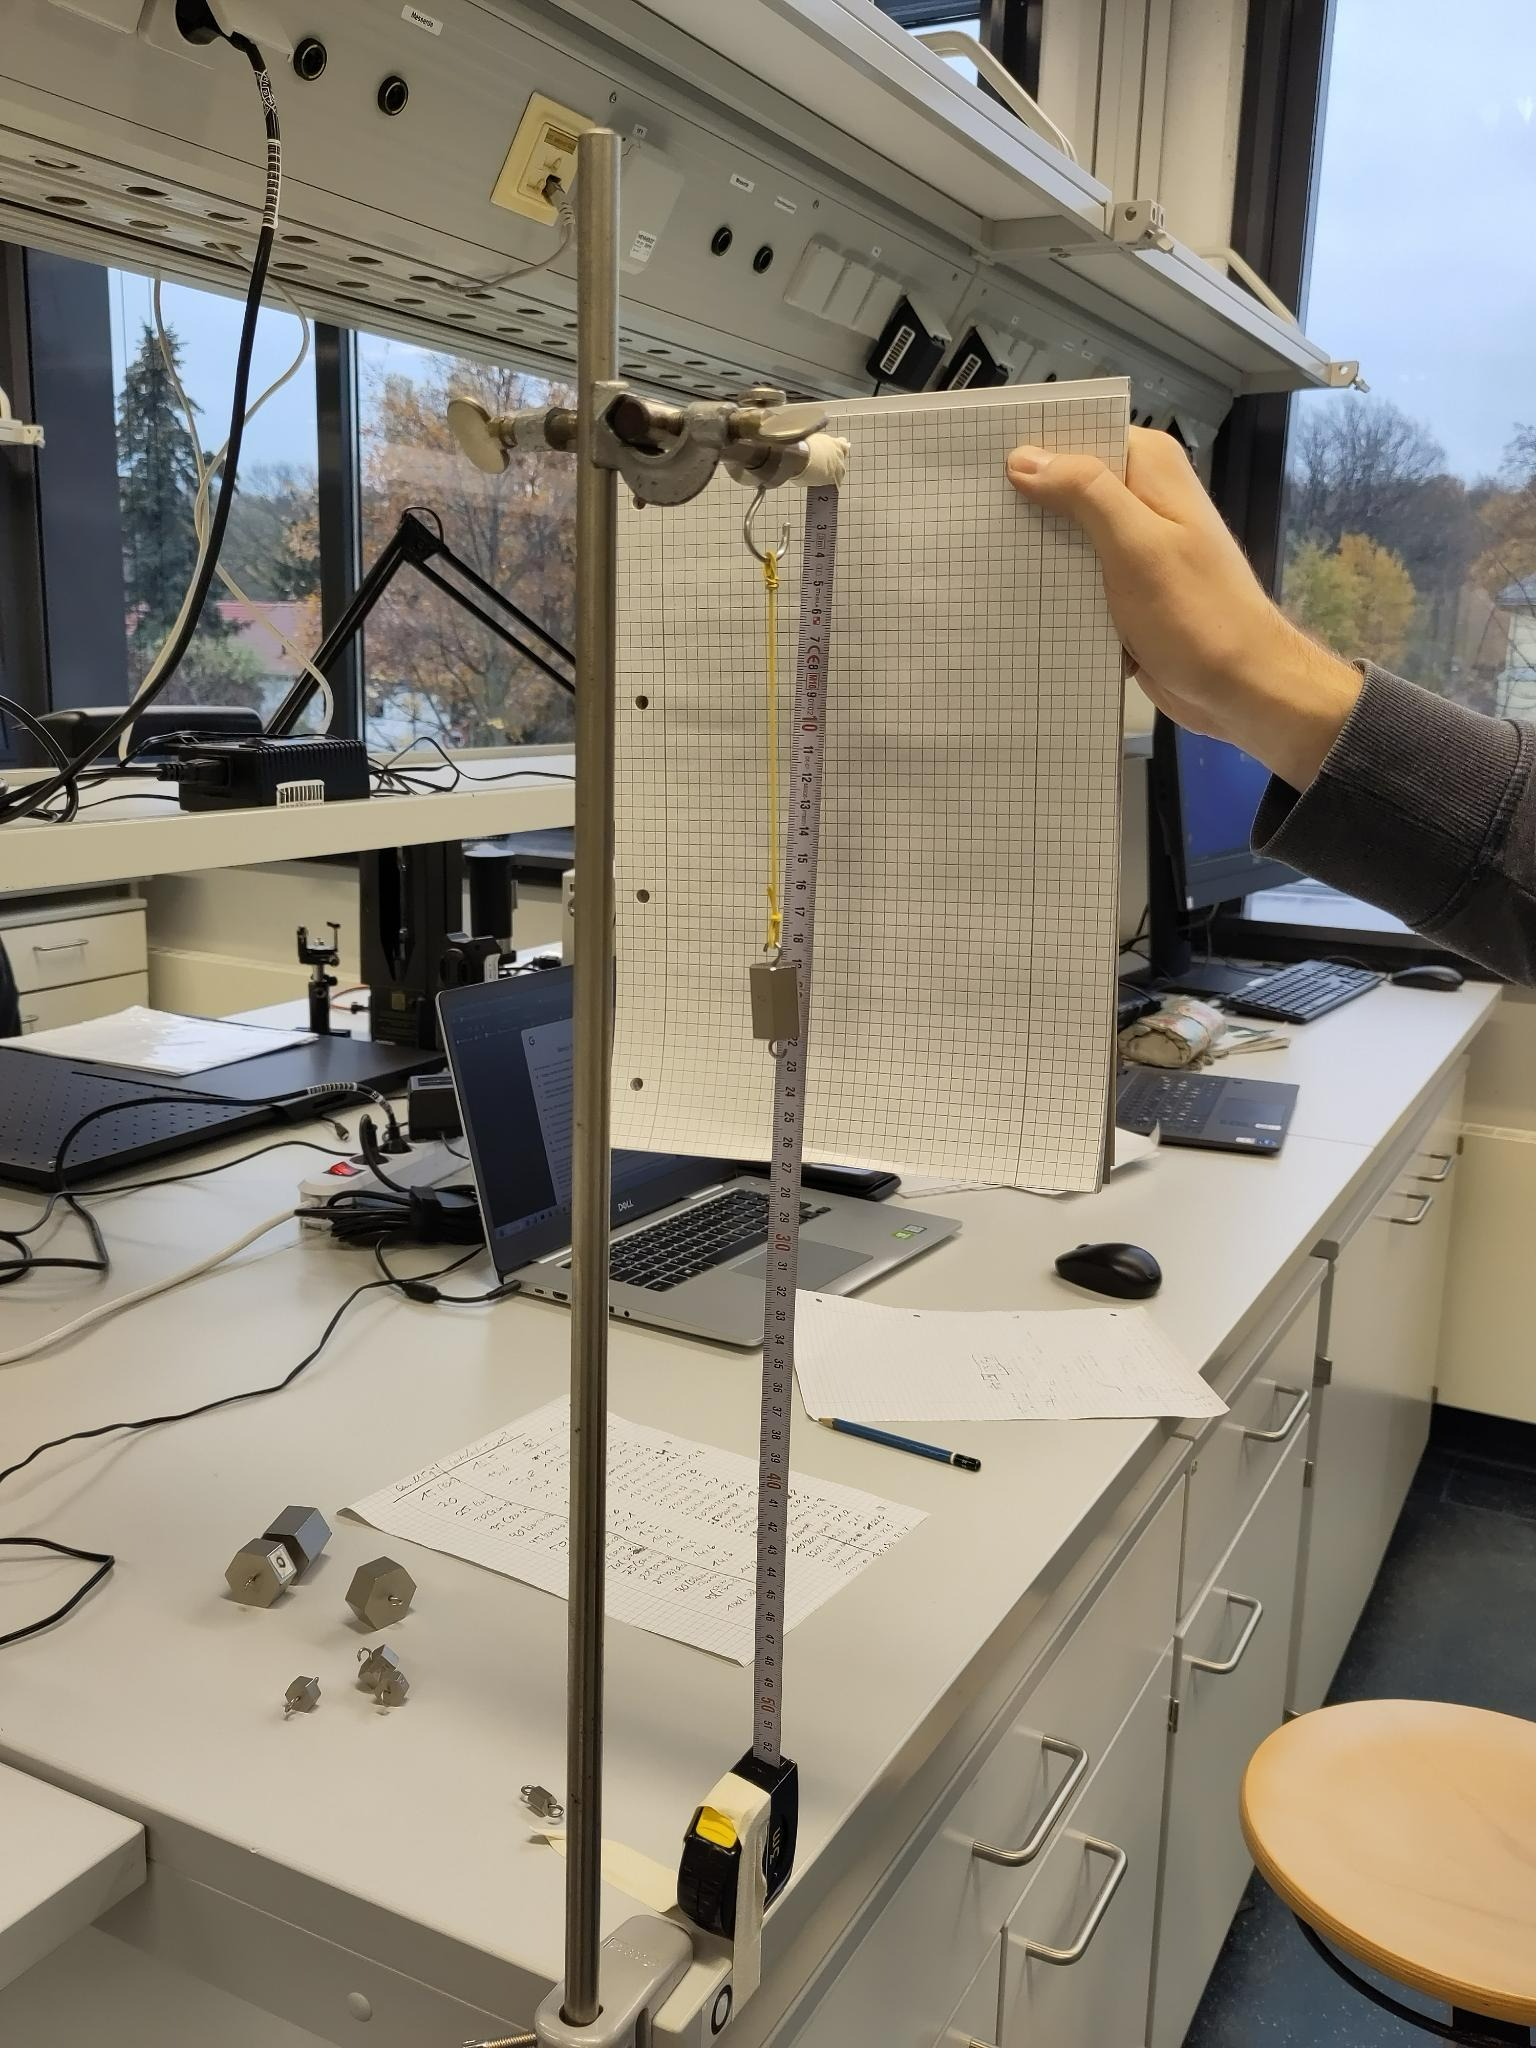
\includegraphics[width=\textwidth,height=0.2\textheight]{Bilder/V2B2.jpeg}
\caption{Versuchsaufbau 2, Nahansicht}
\end{figure}

\hypertarget{durchfuxfchrung-1}{%
\subsection{Durchführung}\label{durchfuxfchrung-1}}

Analog zu Versuch 1. Wir haben uns dafür entschieden bis zur Marke von
100g in 5g - Intervallen und danach in 10g- Schriiten zu messen, um die
Daten mit den Daten aus der ersten Versuchsreihe gut vergleichen können.
Da das Band allerdings viel stärker durch das Anbringen von Gewicht
gedehnt wurde, konnten wir ab 360g keine Messungewn mehr durchführen, da
die Gewichte durch ihre Länge anfingen am Tisch aufzuliegen und so die
Normalkraft die Gewichtskraft verfälscht hätte. Stattdessen haben wir
den aus platztechnisch noch gut messbaren Wert für 400g genommen und den
Rest der Tabelle nicht ausgefüllt. \(x_0\) lag bei uns in diesem Fall
bei 15,8cm.

\hypertarget{fehlerquellen-1}{%
\subsection{Fehlerquellen}\label{fehlerquellen-1}}

Ein möglicher Faktor, der die Federkonstane verfälschen kann, ist neben
den im Versuch 1 genannten Problemen, die Art der Befestigung des nun
einsträngigen Gummibandes. Diese geschaf in Form eines Knotens am Haken.
Dabei wurde ein Teil des Gummibandes verwendet, der im folgenden Versuch
dann nicht gedehnt wurde.

\hypertarget{messung-1}{%
\subsection{Messung}\label{messung-1}}

Auch hier wurden die gemessenen Längen in die gleiche csv-Datei
gespeichert, wie in Versuch 1. Die Massen der Gewichte sind ebenfalls
bekannt. Die Unsicherheiten der Waage und der Skala (Maßband) könen
ebenfalls übernommen werden, da es sich um die selben Geräte handelt. Da
die Massen dieselben sind sind auch die Gewichtskräfte und deren
Unsicherheiten dieselben.

\hypertarget{auswertung}{%
\subsection{Auswertung}\label{auswertung}}

Die Elongation muss erneut berechnet werden. Dafür wird die
Anfangsausdehnung \(x_0\) von den Ausdehnungen \(x_i\) abgezugen und in
Meter umgerechnet werden.

Die Federkonstante wird gemäß Gleichung \ref{hook:eq:Federkonstante}
berechnet. Ebenso deren Unsicherheiten für jeden einzelnen Wert gemäß
Gleichung \ref{hook:eq:u_Federkonstante}. Die Berechnung erfolgt mit
Hilfe der Funktion ``u\_D\_funktion'', welche in Versuch 1 definiert
wurde.

\begin{Shaded}
\begin{Highlighting}[]
\CommentTok{\# Entfernen von NA{-}Zeilen. Die Werte werden aus dem in Versuch 1 erstellten }
\CommentTok{\# Dataframe kopiert}
\NormalTok{Messreihe2 }\OtherTok{\textless{}{-}}\NormalTok{ Messreihe[}\FunctionTok{complete.cases}\NormalTok{(Messreihe[ ,}\FunctionTok{c}\NormalTok{(}\DecValTok{5}\NormalTok{,}\DecValTok{14}\NormalTok{,}\DecValTok{15}\NormalTok{)]),]}
\CommentTok{\# Normierung der Auslenkung}
\NormalTok{Messreihe2}\SpecialCharTok{$}\NormalTok{Auslenkung2\_x0 }\OtherTok{\textless{}{-}}\NormalTok{ Messreihe2}\SpecialCharTok{$}\NormalTok{Auslenkung2}\FloatTok{{-}15.8}
\CommentTok{\# Umrechnung in m}
\NormalTok{Messreihe2}\SpecialCharTok{$}\NormalTok{Auslenkung2\_x0\_m }\OtherTok{\textless{}{-}}\NormalTok{ Messreihe2}\SpecialCharTok{$}\NormalTok{Auslenkung2\_x0}\SpecialCharTok{/}\DecValTok{100} \CommentTok{\#cm {-}\textgreater{} m}

\CommentTok{\# Berechnung der Federkonstanten}
\NormalTok{Messreihe2}\SpecialCharTok{$}\NormalTok{Federkonstante2 }\OtherTok{\textless{}{-}}\NormalTok{ Messreihe2}\SpecialCharTok{$}\NormalTok{Gewicht\_kg}\SpecialCharTok{*}\NormalTok{g}\SpecialCharTok{/}\NormalTok{Messreihe2}\SpecialCharTok{$}\NormalTok{Auslenkung2\_x0\_m}

\CommentTok{\# Berechnung der Unsicherheit der Federkonstanten}
\NormalTok{Messreihe2}\SpecialCharTok{$}\NormalTok{u\_Federkonstante2 }\OtherTok{\textless{}{-}} \FunctionTok{u\_D\_funktion}\NormalTok{(}\AttributeTok{x=}\NormalTok{Messreihe2}\SpecialCharTok{$}\NormalTok{Auslenkung2\_x0\_m, }
                                           \AttributeTok{m=}\NormalTok{Messreihe2}\SpecialCharTok{$}\NormalTok{Gewicht\_kg,}
                                           \AttributeTok{UM=}\NormalTok{Messreihe2}\SpecialCharTok{$}\NormalTok{u\_m)}
\end{Highlighting}
\end{Shaded}

Kraft-Auslenkung Diagramm:

\begin{center}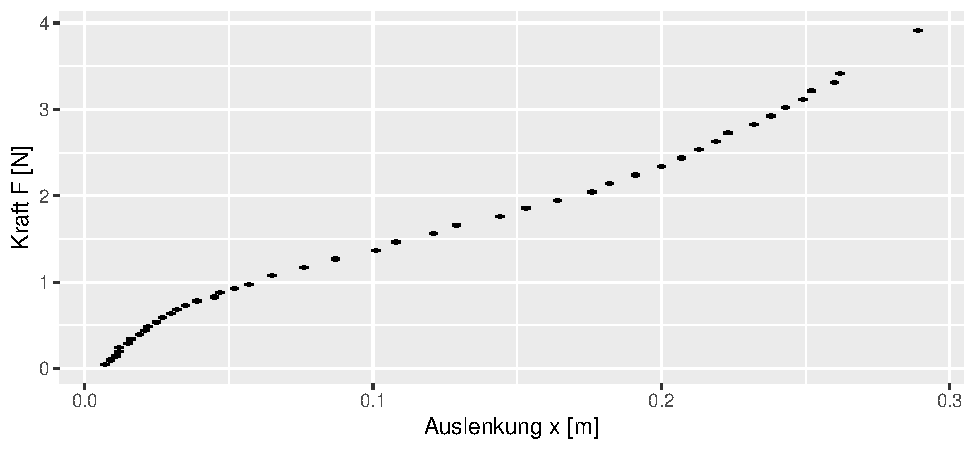
\includegraphics{DehnbareStoffe_files/figure-latex/unnamed-chunk-14-1} \end{center}

Federkonstante-Auslenkung Diagramm:

\begin{center}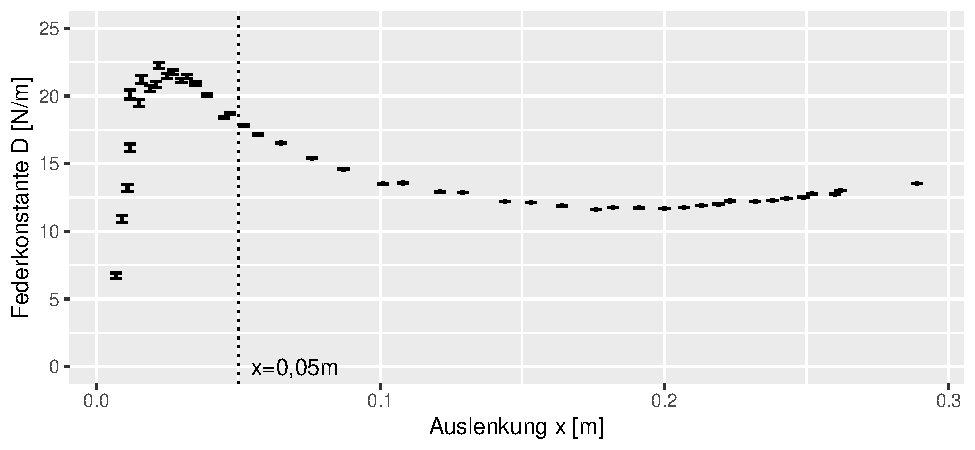
\includegraphics{DehnbareStoffe_files/figure-latex/unnamed-chunk-15-1} \end{center}

Sowohl aus Gründen der Vergleichbarkeit werden auch bei der Berechnung
eines Mittelwertes der Federkonstante in diesem Versuch die Werte für
\(x_i<0,05m\) verworfen. Zudem wird in dem
Federkonstante-Auslenkung-Schaubild auch deutlich, dass für die Werte
kleiner als \textasciitilde5cm Auslenkung die Federkonstante keinen
Stabilen Wert annimmt. Berechnung des Mittelwertes, der
Standardabweichung und der Standardabweichung des Mittelwertes gemäß der
Formeln \ref{Mittelwert}, \ref{Standardabweichung},
\ref{StandardabweichungDesMittelwertes}.

\begin{longtable}[]{@{}lr@{}}
\caption{Statistische Größen zur zweiten bestimmten
Federkonstante}\tabularnewline
\toprule()
& Werte \\
\midrule()
\endfirsthead
\toprule()
& Werte \\
\midrule()
\endhead
Mittelwert\_MW & 13.0996077 \\
Standardabweichung\_SD & 1.6907616 \\
SD\_von\_MW & 0.3195239 \\
\bottomrule()
\end{longtable}

Die in Versuch 2 bestimmte Federkonstante für eine Ausdehnung des Gummis
über \(5cm\) beträgt: \(D_2=(13,10 \pm 0,31)\frac{N}{m}\).

\hypertarget{interpretation}{%
\subsection{Interpretation}\label{interpretation}}

Damit ist die Federkonstante \(D_2\) in etwa halb so groß wie \(D_1\).
Für die gleiche Ausdehnung des Gummibandes aus Versuch 2 um eine Strecke
x ist nur etwa die halbe Kraft vonnöten, wie sie für die gleiche
Ausdehnung des ringförmign Gummibandes aus Versuch 1 nötig wäre.

\newpage

\hypertarget{messwerte-und-errechnete-gruxf6uxdfen-1}{%
\subsubsection{Messwerte und errechnete
Größen}\label{messwerte-und-errechnete-gruxf6uxdfen-1}}

Zusammenfassung der Werte aus Versuch 2, Spaltenbenennung analog zur
Benennung in Versuch 1:

\begin{longtable}[]{@{}
  >{\raggedright\arraybackslash}p{(\columnwidth - 18\tabcolsep) * \real{0.0405}}
  >{\raggedleft\arraybackslash}p{(\columnwidth - 18\tabcolsep) * \real{0.0946}}
  >{\raggedleft\arraybackslash}p{(\columnwidth - 18\tabcolsep) * \real{0.0946}}
  >{\raggedleft\arraybackslash}p{(\columnwidth - 18\tabcolsep) * \real{0.1351}}
  >{\raggedleft\arraybackslash}p{(\columnwidth - 18\tabcolsep) * \real{0.0946}}
  >{\raggedleft\arraybackslash}p{(\columnwidth - 18\tabcolsep) * \real{0.0946}}
  >{\raggedleft\arraybackslash}p{(\columnwidth - 18\tabcolsep) * \real{0.0946}}
  >{\raggedleft\arraybackslash}p{(\columnwidth - 18\tabcolsep) * \real{0.1081}}
  >{\raggedleft\arraybackslash}p{(\columnwidth - 18\tabcolsep) * \real{0.1081}}
  >{\raggedleft\arraybackslash}p{(\columnwidth - 18\tabcolsep) * \real{0.1351}}@{}}
\toprule()
\begin{minipage}[b]{\linewidth}\raggedright
\end{minipage} & \begin{minipage}[b]{\linewidth}\raggedleft
n\_m{[}-{]}
\end{minipage} & \begin{minipage}[b]{\linewidth}\raggedleft
m{[}kg{]}
\end{minipage} & \begin{minipage}[b]{\linewidth}\raggedleft
u\_m{[}kg{]}
\end{minipage} & \begin{minipage}[b]{\linewidth}\raggedleft
L2{[}cm{]}
\end{minipage} & \begin{minipage}[b]{\linewidth}\raggedleft
El2{[}m{]}
\end{minipage} & \begin{minipage}[b]{\linewidth}\raggedleft
F{[}N{]}
\end{minipage} & \begin{minipage}[b]{\linewidth}\raggedleft
u\_F{[}N{]}
\end{minipage} & \begin{minipage}[b]{\linewidth}\raggedleft
D2{[}N/m{]}
\end{minipage} & \begin{minipage}[b]{\linewidth}\raggedleft
u\_D2{[}N/m{]}
\end{minipage} \\
\midrule()
\endhead
2 & 1 & 0.0048 & 0.0000577 & 16.5 & 0.007 & 0.0471 & 0.00057 & 2.6160 &
0.2085 \\
3 & 1 & 0.0100 & 0.0000577 & 16.7 & 0.009 & 0.0981 & 0.00057 & 4.6714 &
0.2503 \\
4 & 2 & 0.0148 & 0.0001155 & 16.9 & 0.011 & 0.1452 & 0.00113 & 6.3125 &
0.2611 \\
5 & 1 & 0.0198 & 0.0000577 & 17.0 & 0.012 & 0.1942 & 0.00057 & 8.0932 &
0.2739 \\
6 & 2 & 0.0246 & 0.0001155 & 17.0 & 0.012 & 0.2413 & 0.00113 & 9.2818 &
0.3482 \\
7 & 2 & 0.0298 & 0.0001155 & 17.3 & 0.015 & 0.2923 & 0.00113 & 11.2438 &
0.2706 \\
8 & 3 & 0.0346 & 0.0001732 & 17.4 & 0.016 & 0.3394 & 0.00170 & 12.5713 &
0.2857 \\
9 & 3 & 0.0398 & 0.0001732 & 17.7 & 0.019 & 0.3904 & 0.00170 & 13.9442 &
0.2341 \\
10 & 4 & 0.0446 & 0.0002309 & 17.9 & 0.021 & 0.4375 & 0.00227 & 15.0871
& 0.2259 \\
11 & 1 & 0.0499 & 0.0000577 & 18.0 & 0.022 & 0.4895 & 0.00057 & 17.4828
& 0.2039 \\
12 & 2 & 0.0547 & 0.0001155 & 18.3 & 0.025 & 0.5366 & 0.00113 & 18.5037
& 0.1776 \\
13 & 2 & 0.0599 & 0.0001155 & 18.5 & 0.027 & 0.5876 & 0.00113 & 19.5873
& 0.1666 \\
14 & 3 & 0.0647 & 0.0001732 & 18.8 & 0.030 & 0.6347 & 0.00170 & 20.4744
& 0.1520 \\
15 & 2 & 0.0699 & 0.0001155 & 19.0 & 0.032 & 0.6857 & 0.00113 & 21.4287
& 0.1385 \\
16 & 3 & 0.0747 & 0.0001732 & 19.3 & 0.035 & 0.7328 & 0.00170 & 22.2063
& 0.1291 \\
17 & 3 & 0.0797 & 0.0001732 & 19.7 & 0.039 & 0.7819 & 0.00170 & 23.6926
& 0.1117 \\
18 & 4 & 0.0845 & 0.0002309 & 20.3 & 0.045 & 0.8289 & 0.00227 & 24.3807
& 0.0961 \\
19 & 4 & 0.0897 & 0.0002309 & 20.5 & 0.047 & 0.8800 & 0.00227 & 25.8811
& 0.0931 \\
20 & 5 & 0.0945 & 0.0002887 & 21.0 & 0.052 & 0.9270 & 0.00283 & 26.4870
& 0.0876 \\
21 & 1 & 0.0995 & 0.0000577 & 21.5 & 0.057 & 0.9761 & 0.00057 & 27.1137
& 0.0609 \\
22 & 2 & 0.1095 & 0.0001155 & 22.3 & 0.065 & 1.0742 & 0.00113 & 27.5435
& 0.0538 \\
23 & 2 & 0.1193 & 0.0001155 & 23.4 & 0.076 & 1.1703 & 0.00113 & 28.5447
& 0.0432 \\
24 & 3 & 0.1293 & 0.0001732 & 24.5 & 0.087 & 1.2684 & 0.00170 & 30.2008
& 0.0388 \\
25 & 4 & 0.1393 & 0.0002309 & 25.9 & 0.101 & 1.3665 & 0.00227 & 31.0576
& 0.0349 \\
26 & 2 & 0.1494 & 0.0001155 & 26.6 & 0.108 & 1.4656 & 0.00113 & 31.8612
& 0.0272 \\
27 & 3 & 0.1594 & 0.0001732 & 27.9 & 0.121 & 1.5637 & 0.00170 & 32.5774
& 0.0256 \\
28 & 3 & 0.1692 & 0.0001732 & 28.7 & 0.129 & 1.6599 & 0.00170 & 31.9202
& 0.0239 \\
29 & 4 & 0.1792 & 0.0002309 & 30.2 & 0.144 & 1.7580 & 0.00227 & 32.5547
& 0.0231 \\
30 & 5 & 0.1892 & 0.0002887 & 31.1 & 0.153 & 1.8561 & 0.00283 & 32.5623
& 0.0244 \\
31 & 1 & 0.1985 & 0.0000577 & 32.2 & 0.164 & 1.9473 & 0.00057 & 31.9227
& 0.0149 \\
32 & 2 & 0.2085 & 0.0001155 & 33.4 & 0.176 & 2.0454 & 0.00113 & 32.4664
& 0.0147 \\
33 & 2 & 0.2183 & 0.0001155 & 34.0 & 0.182 & 2.1415 & 0.00113 & 32.4473
& 0.0144 \\
34 & 3 & 0.2283 & 0.0001732 & 34.9 & 0.191 & 2.2396 & 0.00170 & 31.9946
& 0.0152 \\
35 & 4 & 0.2383 & 0.0002309 & 35.8 & 0.200 & 2.3377 & 0.00227 & 32.0236
& 0.0163 \\
36 & 2 & 0.2484 & 0.0001155 & 36.5 & 0.207 & 2.4368 & 0.00113 & 31.6468
& 0.0126 \\
37 & 3 & 0.2584 & 0.0001732 & 37.1 & 0.213 & 2.5349 & 0.00170 & 31.2951
& 0.0137 \\
38 & 3 & 0.2682 & 0.0001732 & 37.7 & 0.219 & 2.6310 & 0.00170 & 30.5935
& 0.0134 \\
39 & 4 & 0.2782 & 0.0002309 & 38.1 & 0.223 & 2.7291 & 0.00227 & 31.0130
& 0.0150 \\
40 & 5 & 0.2882 & 0.0002887 & 39.0 & 0.232 & 2.8272 & 0.00283 & 31.0686
& 0.0161 \\
41 & 2 & 0.2980 & 0.0001155 & 39.6 & 0.238 & 2.9234 & 0.00113 & 30.1379
& 0.0114 \\
42 & 3 & 0.3080 & 0.0001732 & 40.1 & 0.243 & 3.0215 & 0.00170 & 30.2148
& 0.0124 \\
43 & 3 & 0.3178 & 0.0001732 & 40.7 & 0.249 & 3.1176 & 0.00170 & 30.2681
& 0.0122 \\
44 & 4 & 0.3278 & 0.0002309 & 41.0 & 0.252 & 3.2157 & 0.00227 & 29.7752
& 0.0135 \\
45 & 5 & 0.3378 & 0.0002887 & 41.8 & 0.260 & 3.3138 & 0.00283 & 29.8542
& 0.0147 \\
46 & 3 & 0.3479 & 0.0001732 & 42.0 & 0.262 & 3.4129 & 0.00170 & 29.6774
& 0.0119 \\
51 & 4 & 0.3990 & 0.0002309 & 44.7 & 0.289 & 3.9142 & 0.00227 & 29.4300
& 0.0122 \\
\bottomrule()
\end{longtable}

\end{document}
